\chapter{The Level-1 trigger upgrade jet algorithm}
\label{chap:l1trig}

\section{The Calorimeter Trigger upgrade for Run~2}
\label{sec:trigUpgrade}

With the advent of Run~2 of the \LHC, the demands placed on the \CMS
trigger greatly increased. After a long period of shutdown (known as
\ac{LS1}) the energy
of proton collisions was increased to $13~\tev$ and the bunch crossing
rate decreased to 25~ns. With this configuration the design luminosity
of $10^{34}$cm$^{-2}$s$^{-1}$ can be reached with an average \PU of
around 25 events per bunch crossing. However, the potential luminosity
of the \LHC after the \ac{LS1} upgrade exceeds the original design
value, allowing a \PU of up to 40 simultaneous collisions. The
original Level-1 trigger was not designed to deal with this amount of
\PU. The presence of extra collisions in each event results in a
general increase in the average energy deposited in the calorimeters
of the detector. This extra energy smears out the measurement of
energy deposited by particles from the hard scatter, reducing the
resolution with which it is measured. This acts to increase the rate
at which the trigger accepts events and decrease the accuracy with
which it identifies interesting events. As this rate is limited by the
readout capability, a trigger that is not upgraded will have a reduced
efficiency of acceptance of interesting physics events.  It is
therefore very advantageous to upgrade the Level-1 trigger in a way
that allows it to deal with the extra \PU \cite{Tapper:1556311}.

Along with maintaining a low output rate for a high efficiency,
another key consideration for the Level-1 trigger is the time taken
for
the algorithms to run on the boards that carry out the trigger
processing, their \emph{latency}. This must be kept low to ensure that
every bunch
crossing is analysed in as much detail as possible. To be able to
carry out this sort of processing, the Level-1 trigger makes use of custom
\FPGA boards, as described in Sec.~\ref{sec:triggers}. The complexity
and structure of the trigger algorithms is limited to ensure
they can run quickly enough on the \FPGA boards. An upgrade to the
trigger hardware therefore allows more sophisticated algorithms to be
carried out, while still being able to process every bunch crossing.

The amount of calorimeter information that can be processed by a
single \FPGA is also limited by its input and output capacity. To pass
the full calorimeter data from a single bunch crossing through an
\FPGA in the Level-1 trigger it takes the equivalent of $\sim10$ bunch
crossings of time. In Run~1 of the \LHC, the calculations for
triggering on the calorimeters were performed with the \GCT
\cite{Khachatryan:2016bia}. The \GCT dealt with this delay by
processing different sections of the calorimeter in separate boards,
necessitating duplication of information at the detector section
boundaries. However, by time multiplexing the calorimeter data, it is
possible to have individual \FPGA boards that each process one bunch
crossing with minimal information duplication. To achieve this, 10
\FPGA boards are utilised in a round-robin configuration. The data
collected from the first bunch crossing is processed by one board, the
data from the second bunch crossing by another board and so on. Each
bunch crossing is processed by another board until the first board has
finished and can subsequently process the next available bunch
crossing. This would not be possible without the timing information
provided by time multiplexing the data. As well as increasing the
total possible information bandwidth, this allows greater flexibility
in the algorithms used as each \FPGA has access to the full event
information \cite{1748-0221-9-10-C10034,1748-0221-7-01-C01060}. The
upgrade architecture of the Level-1 trigger is therefore that of a
\TMT, a representation of the difference between this architecture and
that of the \ac{GCT} can be seen in Fig.~\ref{fig:tmt}. The hardware
is also upgraded, exploiting the recent technological improvement in
the performance of \FPGA processors and high-speed optical links
\cite{tp}.

\begin{figure}
  \centering
  \subfloat[Run~1 trigger architecture.]{
    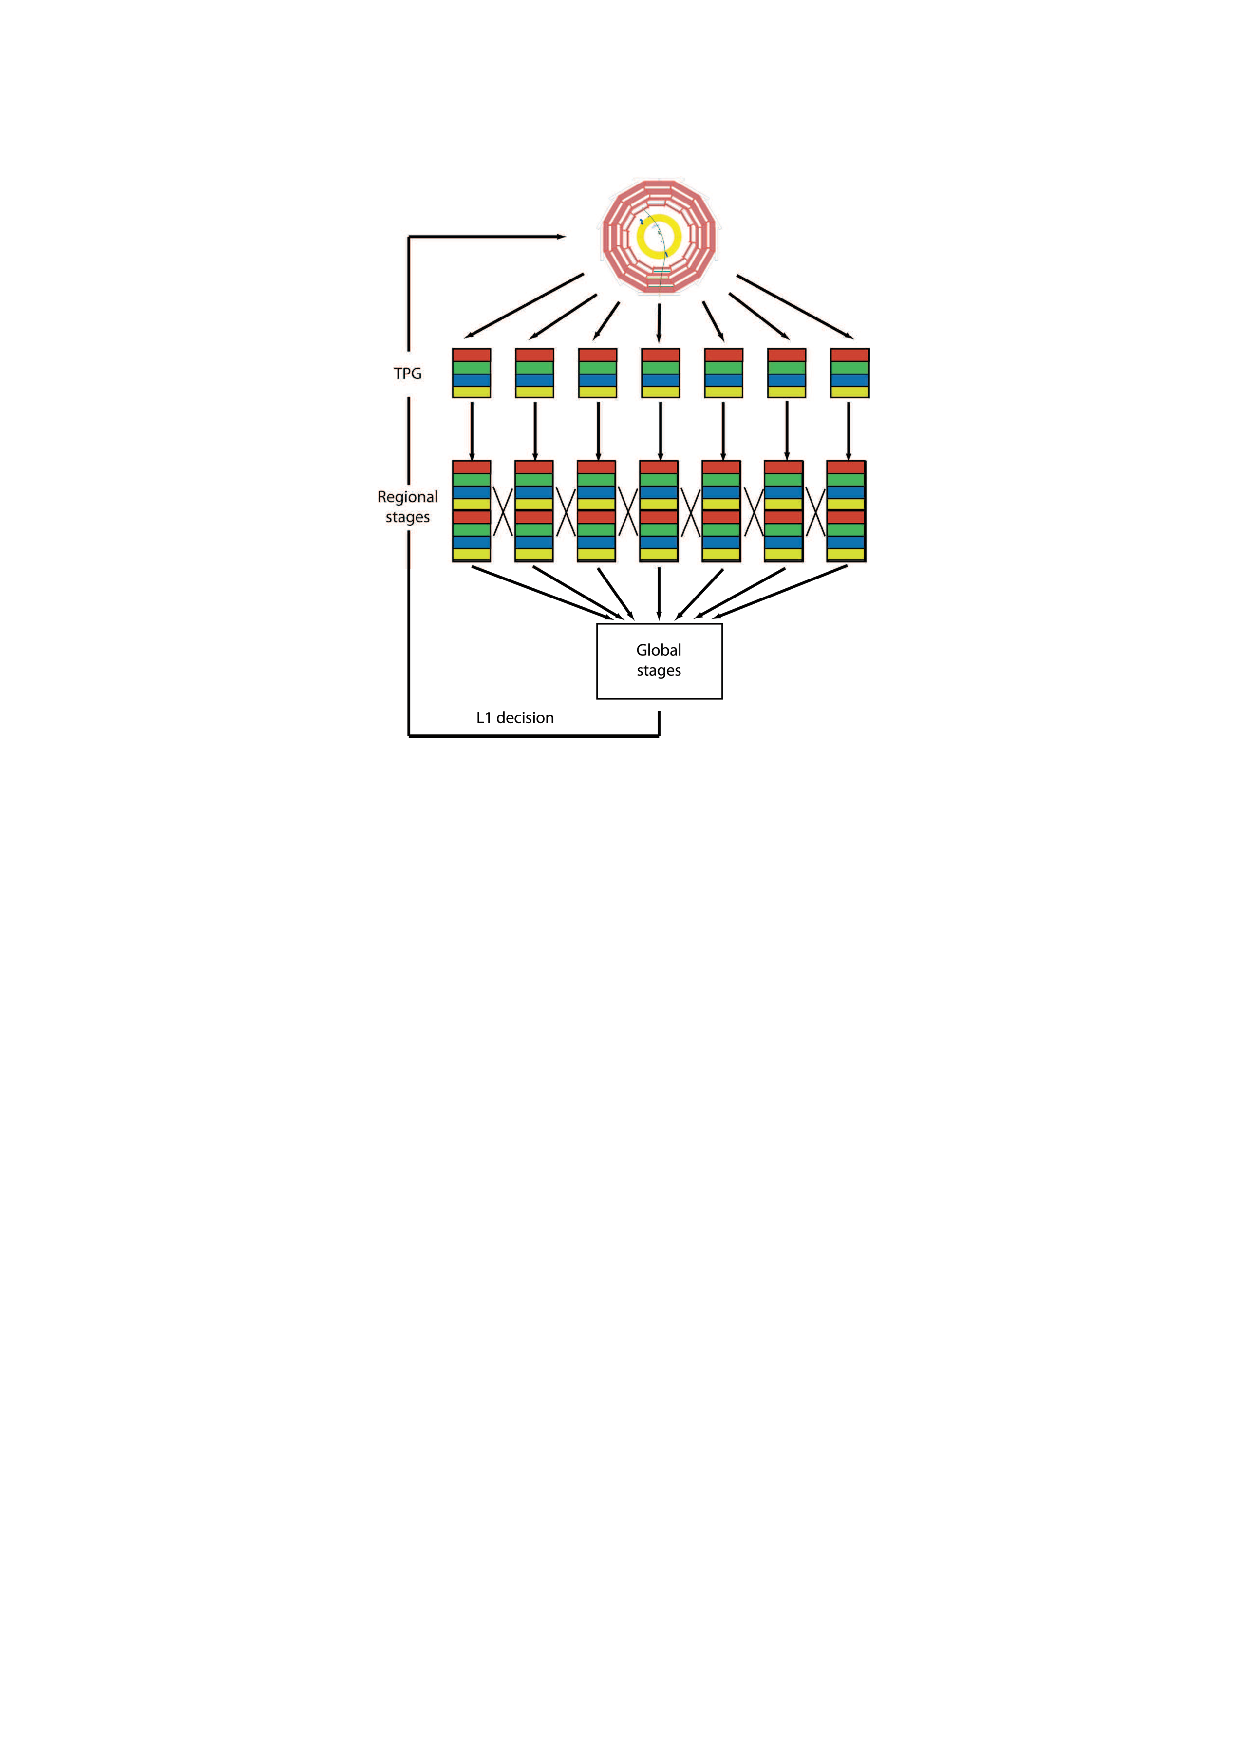
\includegraphics[width=0.4\textwidth]{figs/trigger/old_trigger}
  }~~
  \subfloat[Run~2 upgrade TMT trigger architecture.]{
    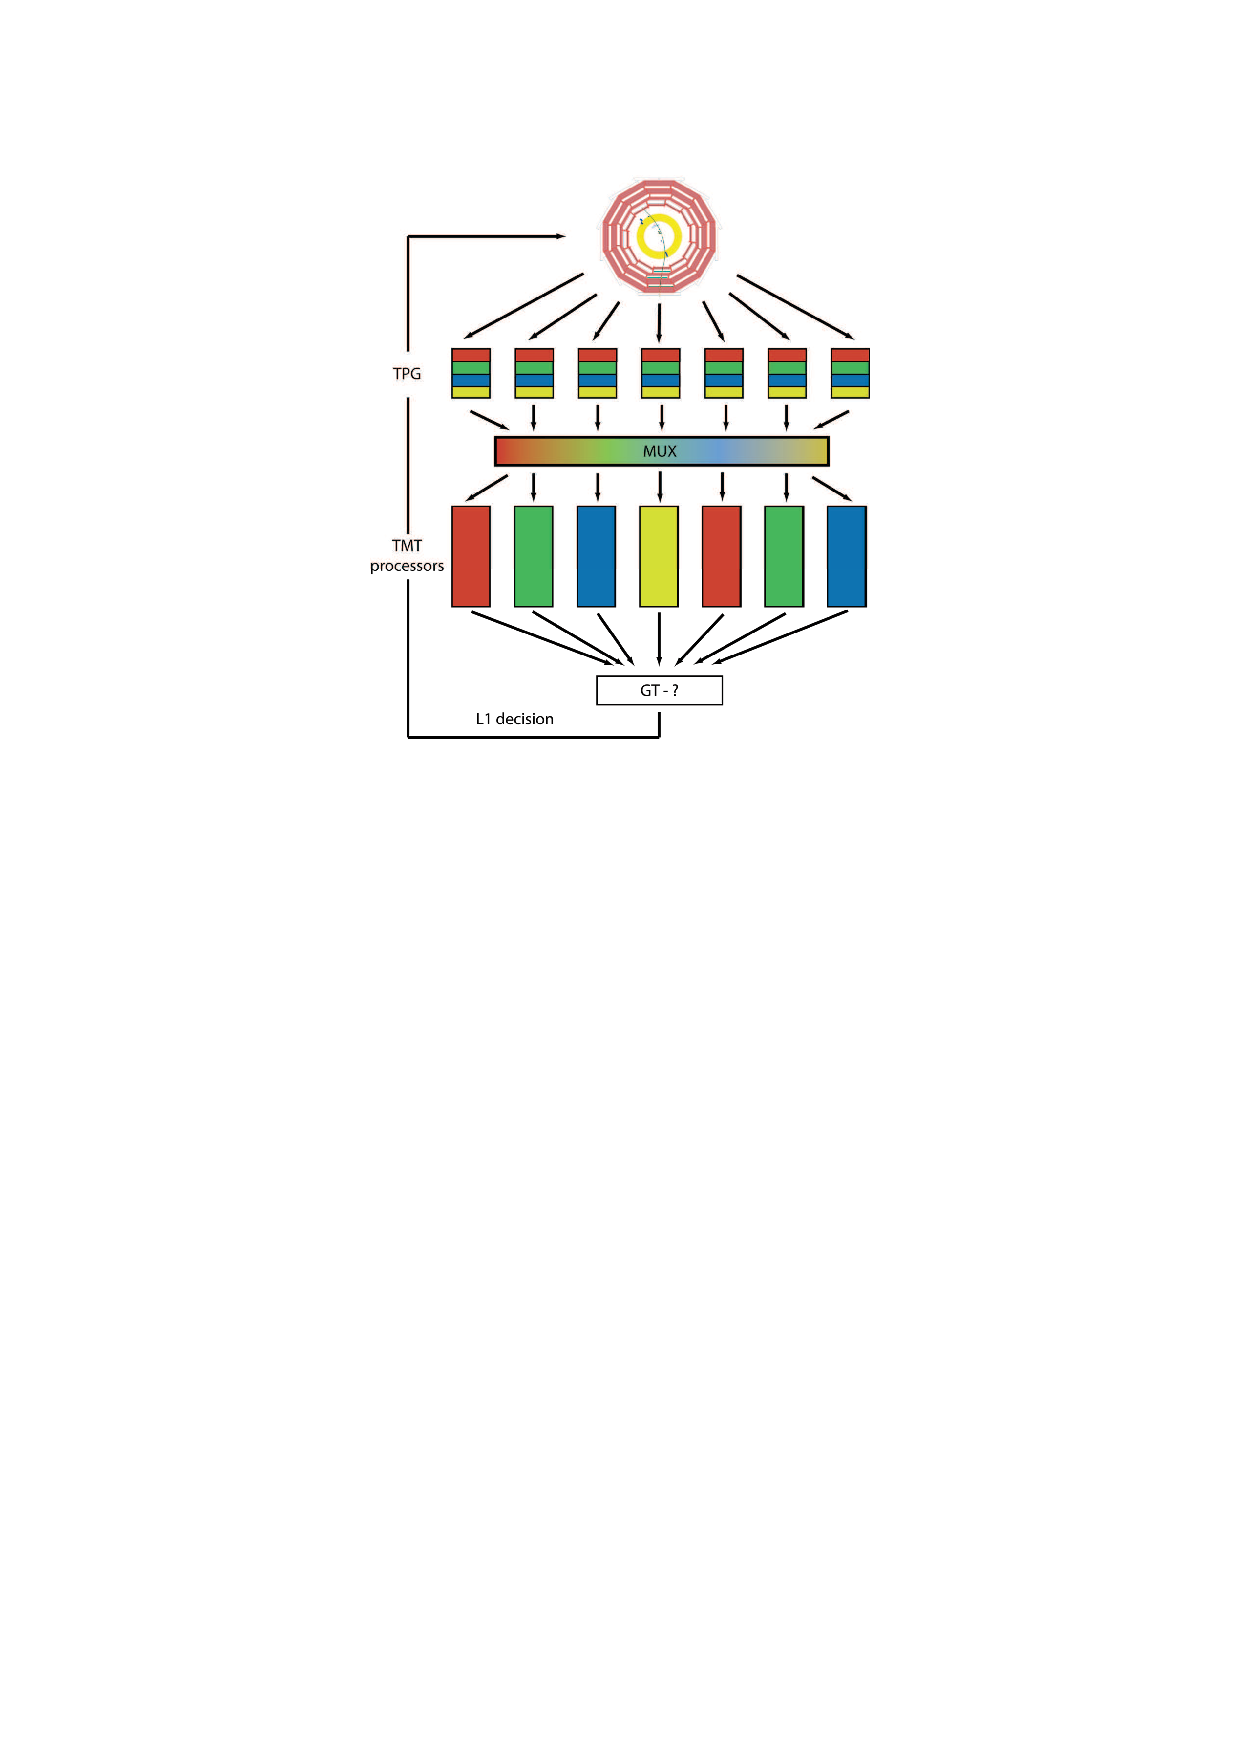
\includegraphics[width=0.4\textwidth]{figs/trigger/tmt}
  } \\
  \caption{A representation of the time multiplexed trigger (TMT)
  architecture (b) as opposed to the pre-upgrade trigger architecture
  (a). The entire information for one event is processed by one board
  rather than just parts of the detector for each board \cite{1748-0221-9-10-C10034}}
  \label{fig:tmt}
\end{figure}

The inputs to the Calorimeter Trigger from the various \ECAL and \HCAL
components are split into a $56\times 72$ grid of \TTs in $\eta$ and
$\phi$ within the barrel and endcap region ($|\eta|<3$), with each
tower covering the area of $5\times5$ \ECAL crystals.  As the
processing power of the \ac{GCT} was limited, for trigger calculations
the \TTs were grouped into $4\times4$ blocks, known as \emph{\ac{RCT}
regions} \cite{Khachatryan:2016bia}. These different regions are
visually represented in Fig.~\ref{fig:trigger_calorimeter}. Due to the
advantages brought by the upgrade, the new algorithms have access
to the full granularity information of all the \TTs. A representation
of the upgrade to the spatial resolution afforded by this change is
in Fig.~\ref{fig:sunnyJim}.

\begin{figure}
	\begin{center}
		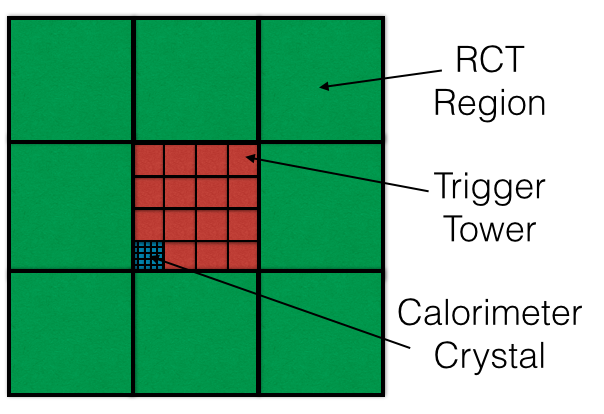
\includegraphics[width=0.5\linewidth]{figs/trigger/trigger_calorimeter}
	\end{center}
	\caption{The breakdown of the different calorimeter regions, the
  \ac{RCT} regions
  and trigger towers are both shown within the context of the \ECAL
  calorimeter crystals.}
	\label{fig:trigger_calorimeter}
\end{figure}

\begin{figure}
  \centering
  \subfloat[Run~1 calorimeter trigger resolution.]{
    
\includegraphics[width=0.35\textwidth]{figs/trigger/L1inputreslegacy}
  }~~
  \subfloat[Run~2 upgrade calorimeter trigger resolution.]{
    
\includegraphics[width=0.35\textwidth]{figs/trigger/L1inputresupgrade}
  } \\
  \caption{A representation of the spatial resolution of the trigger
  inputs to the calorimeter trigger for the Level-1 trigger before and
  after the upgrade.}
  \label{fig:sunnyJim}
\end{figure}

\section{The jet finder and energy sums}
\label{sec:jetFinder}

To make use of the potential brought by the Level-1 trigger upgrade,
new trigger algorithms are developed to improve the selection of
interesting physics processes. With a better view of the substructure
of energy deposits within the calorimeters, the identification of three
pronged tau jets and isolated electrons can be significantly improved,
for example \cite{egllr,taullr}. 

One area in which algorithm improvements can have a significant impact
is in the jet finding algorithm. As the Level-1 trigger must be of a
fixed latency, it cannot make use of an iterative algorithm such as
those used during offline jet-finding (described in
Sec.~\ref{sec:jets_reco}). In the algorithm used during Run~1, the jet
candidates are created from a $3\times3$ \ac{RCT} region sliding
window.  Candidates in which the central region has the maximum energy
are kept as jets \cite{Chatrchyan:2008aa}. These jets cover an area of
$\Delta\eta\times\Delta\phi = 1.04 \times 1.04$, which matches
reasonably well the area covered by circular jets with $R=0.5$, the
maximum radius for Run~1 offline jets.  To help mitigate the
reconstruction of jets originating from \PU, the central region of the
jet finder is also required to exceed a minimum energy, known as the
\emph{seed threshold}. Due to latency and processing power
constraints, there is no way in which contribution to the energy of
the jet from \PU can be subtracted dynamically. Along with the relatively
large jet size, this means the performance of the algorithm will be
severely reduced by the conditions present during Run~2. An upgrade
provides the extra processing power to carry out a dynamic \PUS,
correcting the energy of each jet from the influence of \PU. The
increased position resolution will also allow for a more accurate
determination of the direction of the jets.

Once a jet algorithm is chosen, the jets can be used to make Level-1
trigger decisions. This typically involves selecting events that are
observed to have jets, or sums of jets, with an energy above a certain
threshold. The selection made within the Level-1 trigger is
designed to pick out interesting physical processes, while removing
background events. The particular configuration of jets that lead
to an acceptance of an event is known as a \emph{trigger}. For
example, a single-jet trigger would require at least one jet above a
certain \pT threshold, or a quad-jet trigger would require at least
four jets above a certain threshold. The performance of the Level-1
trigger algorithms are therefore typically measured within this
context, as discussed in Sec.~\ref{sec:jet_algo_performance}.  When
designing these triggers, the total rate of acceptance of the Level-1
trigger cannot exceed a predefined value $\sim 100$~kHz. The sum of
the rates of all the trigger decisions must be kept below this number.
A trade off between all the potential triggers must be made, making it
of utmost importance to design triggers with manageable rates.

\subsection{The upgraded jet algorithm}
\label{sec:stage2_jetalgo}

The jet algorithm for the Run~2 CMS trigger upgrade operates on
the sum of the \ECAL and \HCAL energy deposits in the \TTs. The studies
in this Chapter consider the \TTs within $|\eta|<3$.
% , with the potential
% to extend the algorithm up to $|\eta|<5$. 

Starting with a similar idea as in Run~1, the upgrade makes use of a
sliding window algorithm. In the upgrade, however, the window
considered is a $9\times9$ square of \TTs, covering
$\Delta\eta\times\Delta\phi = 0.78 \times 0.78$. This odd number of
trigger towers results in an easily defined central tower as well as
matching the area covered by the $R=0.4$ offline jets that are used in
Run~2. Within a window the central tower is considered as the
direction of a candidate jet. The candidate is vetoed if any of the
other \TTs in the square have an energy deposit of either greater than
or greater than or equal to it. The veto condition is
antisymmetric along the diagonal of the square to prevent \TTs with the
same energy from vetoing one another. A representation of the window
considered can be seen in Fig.~\ref{fig:stage2_jetalgo}.  Any \TTs that
pass this criteria are considered as jet centres, where the jet energy
is equal to the sum of all the towers within the $9\times9$ square.
% Taking the highest energy
% TT as the centre of the jet axis is motivated by the fact that jets
% are boosted objects with most of their energy in the middle
% \cite{JetProfile_pileup}.

The veto conditions applied on the central \TT ensure that no two
overlapping jets are reconstructed, avoiding the duplication of energy
deposits. However, the algorithm can introduce inefficiencies in very
specific jet topologies. In these cases a high energy \TT vetoes a
medium energy \TT which then vetoes a lower energy \TT. 
The medium energy \TT is included in the jet constructed by the high energy
\TT, however the lower energy \TT is lost. This is not usually a
problem when making decisions with the Level-1 trigger, as the high
energy \TT will usually ensure that the event is triggered, despite
energy being lost.

\begin{figure}
	\begin{center}
		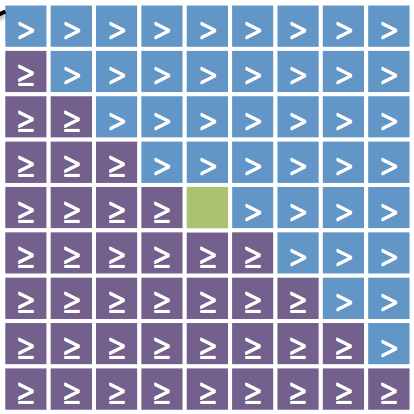
\includegraphics[width=0.3\linewidth]{figs/trigger/stage2_jetalgo}
  \end{center} \caption{The consideration of a Trigger Tower candidate
  for the upgrade Level-1 Trigger jet algorithm. The candidate (green)
  is vetoed if the energy of the other towers meets the condition
  shown in the blue and purple towers.}
	\label{fig:stage2_jetalgo}
\end{figure}

\subsection{A comparison with the offline jet algorithm}

In order to test the performance of the upgrade algorithm it is compared to
jet finding with anti-$k_T$ clustering, the most popular algorithm
for offline jet reconstruction. As the Level-1 algorithm has less
sophisticated inputs than the \PF candidates used offline, the
anti-$k_T$ algorithm is used to find jets with the \TTs as input. The test was
carried out on a $t\bar{t}$ \MC simulation, which contains a high
multiplicity of jets that are produced in top-quark decays. The performance of
the algorithm compared to anti-$k_T$ jet clustering with $R=0.4$ can
be seen in Fig.~\ref{fig:ak4_comp}. For the jet with the highest \pT,
the leading jet, the distributions of \pT and $\eta$ are very similar
for both the jet finding algorithms. For the fourth-leading jet more
differences emerge at low \pT and the edges of the $\eta$
distribution. This is probably due to the ability of the anti-$k_T$
algorithm to adaptively fit smaller radius jets and those at the edge
of the detector acceptance.

\begin{figure}
	\begin{center}
		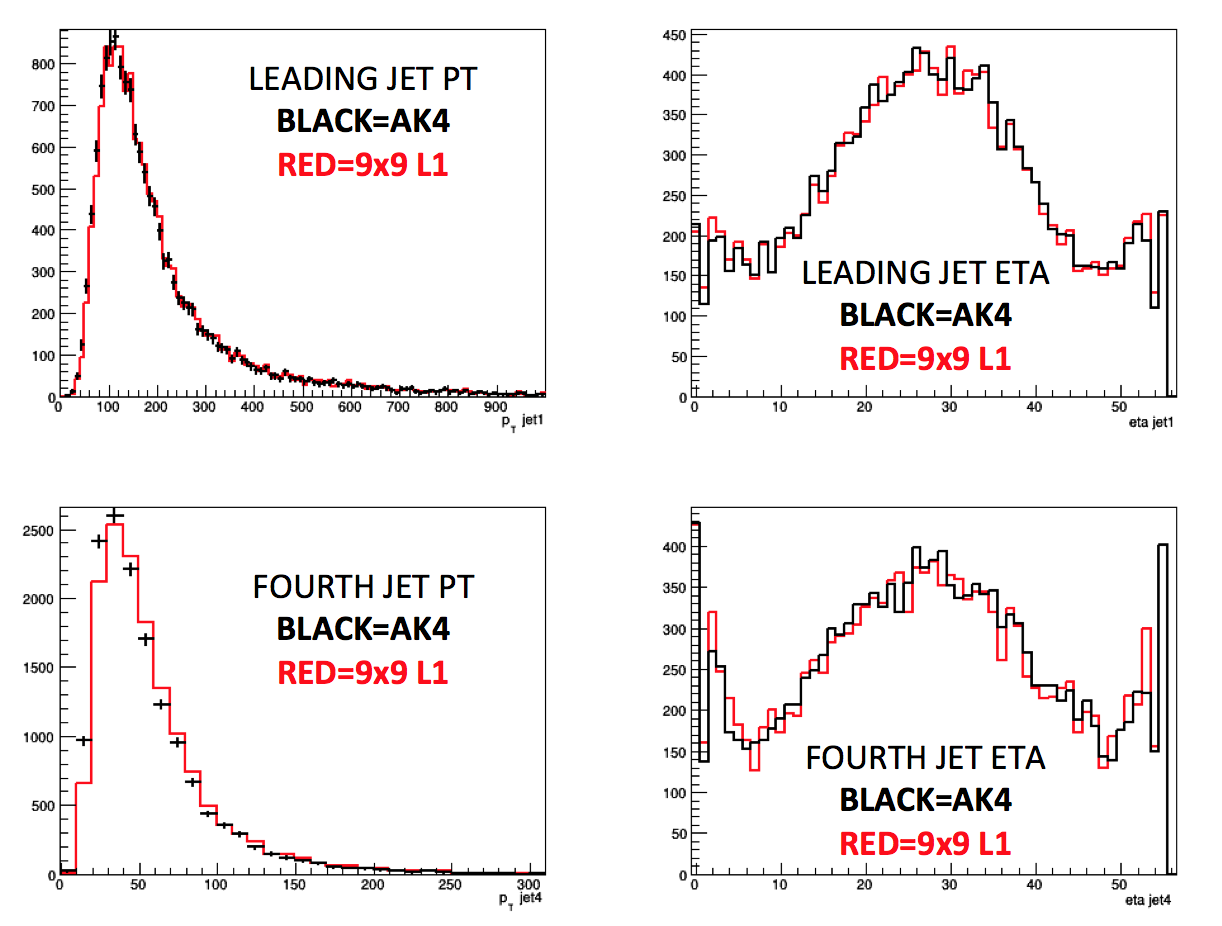
\includegraphics[width=1.0\linewidth]{figs/trigger/jet_l1s2_compak4}
	\end{center}
  \caption{A comparison between the upgrade Level-1 trigger ($9\times9$L1) jet
  algorithm and the anti-$k_T$ offline algorithm with R=0.4 
  (AK4), taking
  the \TTs as input.  These plots are produced from a
  $t\bar{t}$ simulation with $13$~TeV proton collisions and \PU $\sim40$.
  The units for the pseudorapidity are in trigger tower units, which
  range from 0 at $\eta =-3$ to 56 at $\eta=3$.}
	\label{fig:ak4_comp}
\end{figure}

\subsection{Energy sums}

Along with finding jets in an event, the Level-1 trigger is required
to calculate energy sums, analogous to those discussed in
Sec.~\ref{sec:met_reco}.  These energy sums can take either the jets
or \TTs as input. They include:
\begin{itemize}
\item{total $E_T$, the scalar sum of the transverse energy in all the
\TTs}
\item{\met, the inverse vector sum of the transverse energy in all the
\TTs}
\item{\HT, the scalar sum of all the Level-1 jets}
\item{\MHT, the inverse vector sum of all the Level-1 jets}
\end{itemize}

\section{Pileup subtraction}
\label{sec:pus}

\subsection{Characterising pileup}
 
On average, the decays from \PU are expected to be isotropically
distributed around the detector. However, there will be significant
event-by-event differences due to Poisson fluctuations in the number
of \PU collisions. While the number of simultaneous interactions is
such that these fluctuations are significant, it is advantageous to
correct for the \PU on a per-event basis. To be able to remove the
effects of \PU in the Level-1 trigger there needs to be a way to remove
the objects that originate from \PU. Additionally, an
estimate of the average energy deposited in each event should be used
to correct the $E_T$ of the remaining objects. These procedures are
known collectively as \emph{\acf{PUS}}.

It is observed that the density of decays from \PU 
depend on their position in $\eta$ \cite{Cacciari2011}. This is
most likely caused by the differing response of the detector along its
length. The fact that the trigger only has access to
coarse calorimeter information and no tracks means these detector
effects are likely to be enhanced. It is therefore desirable for \PUS
algorithms to measure the \PU energy density near to the objects that
are corrected. This \emph{local} \PUS then requires a trade off
between the proximity to the object and the effects of the
larger statistical fluctuations from sampling a smaller area. 

A \emph{global} subtraction can be used to determine the average
energy density across the whole detector. This method is much less
susceptible to fluctuations and contamination from particles from the
hard-interaction, but does not take account of local fluctuations or
detector effects.

The ideal form of \PUS will remove the dependence of the Level-1
trigger rate and efficiency on the number of simultaneous interactions
in an event. It should do this in a way that improves the resolution
of object energy measurements, increasing the acceptance
of interesting physics events while allowing for the rejection of soft
QCD multijet processes. It is also important to take account of the
Level-1 trigger architecture when designing the algorithm to ensure
that it can be performed with a fixed latency. Different forms of \PUS
in the Level-1 trigger are outlined in this section and their
performance subject to this criteria is is examined in
Sec.~\ref{sec:jet_algo_performance}. 

As well as mitigating \PU from simultaneous collisions, the effects of
\ac{OOTPU} must be removed. This predominantly achieved during the
generation of the \TT inputs for the calorimeter trigger. When reading
out the energy deposited in the \ECAL and \HCAL the average extra
energy deemed to have come from a previous bunch crossing is
subtracted and a correction factor is applied. This mitigation
performs well enough to make the effects of \ac{OOTPU} subdominant
with respect to in-time \PU.

\subsection{Global pileup subtraction}

A prominent method of \PUS is $\rho$-area correction
\cite{Cacciari:2007fd,Cacciari:2008gn}. It works by finding the
average energy per unit area in the calorimeter due to PU, $\rho$, and
subtracting it from each reconstructed jet. A favoured estimator for this
quantity is:
\begin{equation}
\rho\equiv median(\frac{p_{Tj}}{A_j}),
\end{equation}
where $p_{Tj}$ is the transverse momentum of a jet $j$, $A_j$ is its
area and the median is taken over all reconstructed jets in an event.
In the plots in this chapter, this form of \PUS is known as \emph{global}. It
acts to remove half the jets in an event, the low energy half, and
correct down the energy of the remaining half. This works works
particularly well in high \PU cases as $\rho$ is insensitive to
fluctuations in the energy of interesting physics events. 
% It is
% possible to take account of $\eta$ dependence through a new variable
% \emph{local $\rho$}, where the different values are calculated in
% different $\eta$ ranges of the detector. This method loses robustness
% as the number of jets that are sampled is lowered for each $\rho$
% calculation.

The mean value of \rho, as a function of the number of interactions,
is shown in Fig.~\ref{fig:rho}. This is taken from a minimum bias \MC
simulation in which there is no visible hard interaction but only
overlaid \PU collisions. There is a good correlation between the
number of simultaneous collisions and \rho, indicating that it is
indeed a reasonable measure of the \PU in the event. The correlation
also passes through the origin, indicating that \ac{OOTPU} is not a
problem with a 50~ns bunch spacing.

\begin{figure}
	\begin{center}
		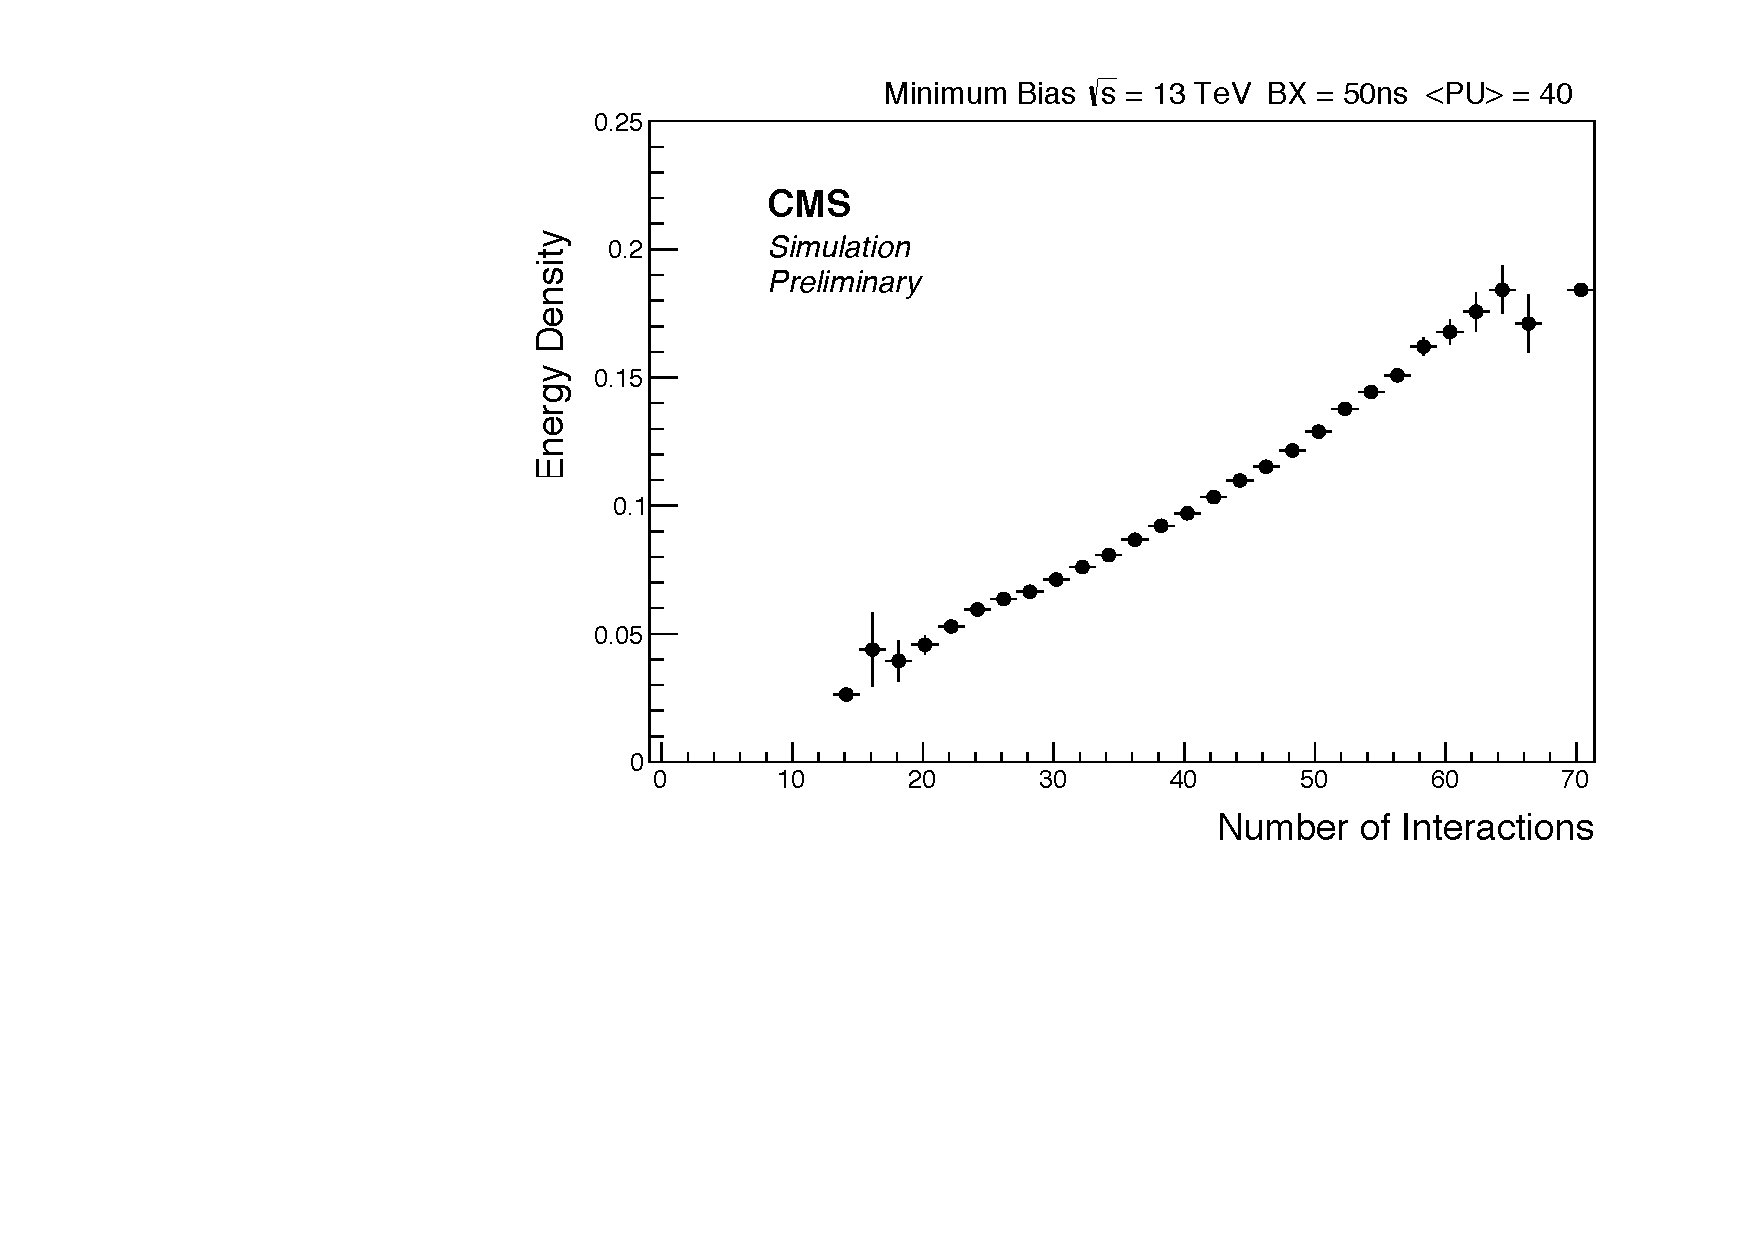
\includegraphics[width=0.8\linewidth]{figs/trigger/median}
  \caption{The median energy density, \rho, of Level-1 jets in the \CMS
  calorimeters as a function of the number of simultaneous collisions.
  This is taken from minimum bias \MC simulation at 13~\tev with a
  50~ns bunch crossing time}
	\label{fig:rho}
	\end{center}
\end{figure}

Subtraction with the $\rho$-area method has a latency penalty when
implemented in hardware as the jets must be found before \rho can be
calculated and subtracted from their energies. Depending on the final
firmware designs this can present a problem and makes global \rho
subtraction harder to perform in hardware. Despite this fact, as
global \rho is a popular and well understood form of offline \PUS it
acts as a good benchmark against which to test other algorithms.

\subsection{Donut Subtraction}

As jets from the hard scatter are typically boosted objects, most of
their energy is deposited very close to the central \TT of the jet
algorithm \cite{JetProfile_pileup}. A typical energy profile of a jet
is shown in Fig.~\ref{fig:jetprofile}. In the case of isolated jets,
the ring five \TTs from the centre of the jet can be assumed to contain
only contamination from \PU.  The \emph{donut subtraction} algorithm therefore take the
energy per unit area in the ring of \TTs surrounding the jet (shown in
Fig.~\ref{fig:donutstrips}) and scales
it up by the area of the jet. The resulting energy is then subtracted
from the jet to correct any \PU contamination. This kind of \PUS has
been applied in the analysis of heavy ion collisions at the \LHC
\cite{Cacciari:2010te}.

\begin{figure}
	\begin{center}
		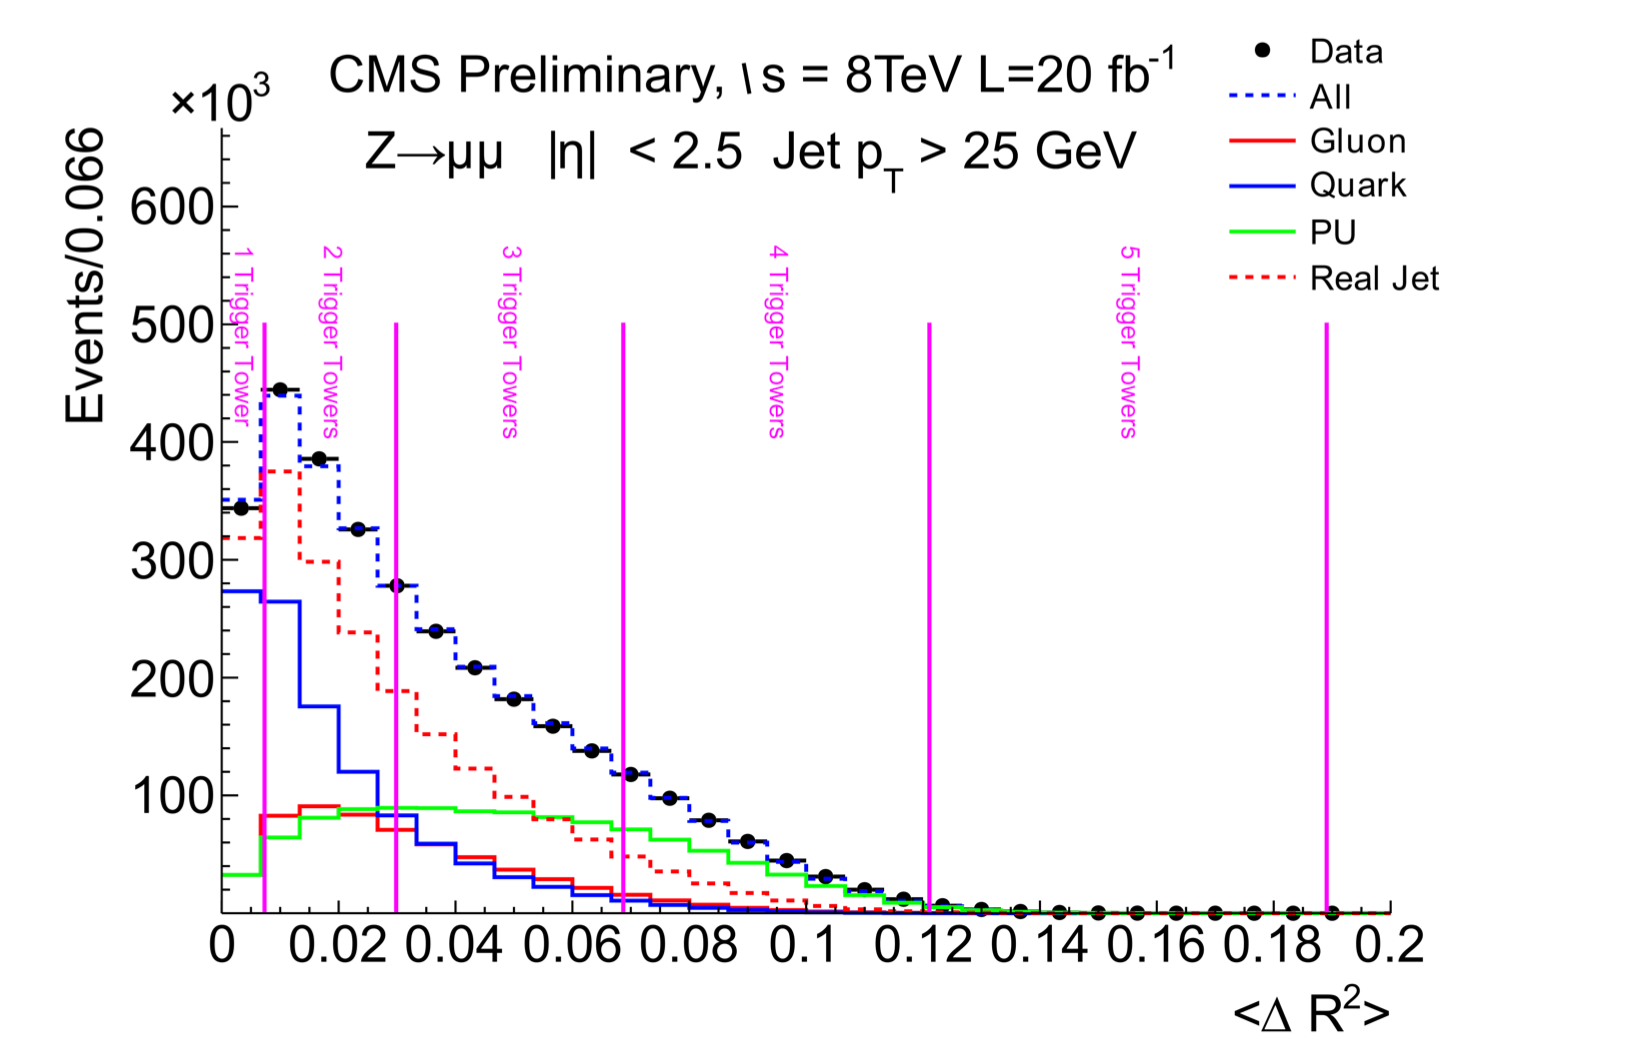
\includegraphics[width=0.8\linewidth]{figs/trigger/jetProfile}
  \caption{ Jet energy profile as a function of distance from the
  centre of the jet, $R$. The number of trigger towers that the
  distances corresponds to are shown in pink. Calculated for jets from
  a simulation of Z to $\mu\mu$ events \cite{JetProfile_pileup}}
	\label{fig:jetprofile}
	\end{center}
\end{figure}

This approach only works for correcting isolated jets, if one jet from
the hard-scatter is
in the vicinity of another, the energy in the donut can be increased to
above that of \PU. To mitigate this, only the median two $4\times1$
\TT strips of the four that make up the donut are used to calculate
the \PU energy density. This reduces the chance that energy from
another jet will be counted as \PU and also removes strips that have
very little energy in them from a downward fluctuation in \PU
contamination. An example of the two strips that could be selected can
be seen in purple in Fig.~\ref{fig:medianstrips}.

\begin{figure}
  \centering
  \subfloat[Strips considered for donut subtraction.]{
    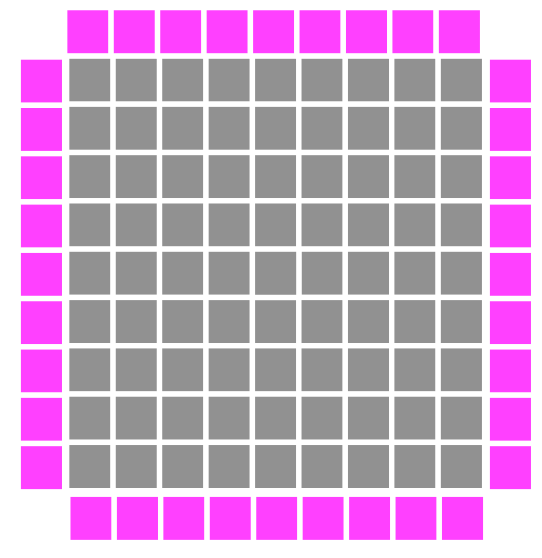
\includegraphics[width=0.3\textwidth]{figs/trigger/donut}
    \label{fig:donutstrips}
  }~ 
  \subfloat[Example of median energy strips.]{
    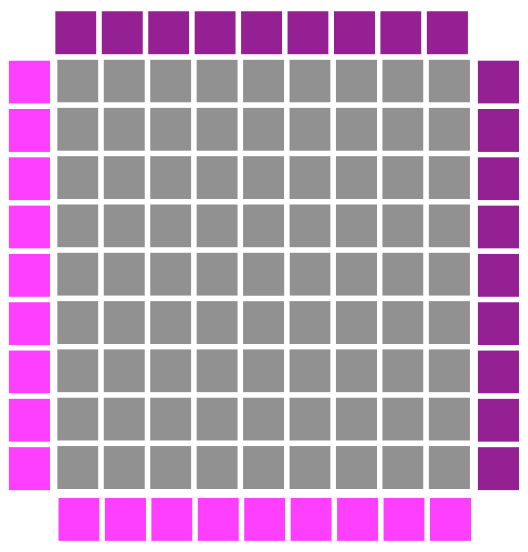
\includegraphics[width=0.3\textwidth]{figs/trigger/donut2}
    \label{fig:medianstrips}
  }~
  \subfloat[Strips considered for chunky donut subtraction.]{
    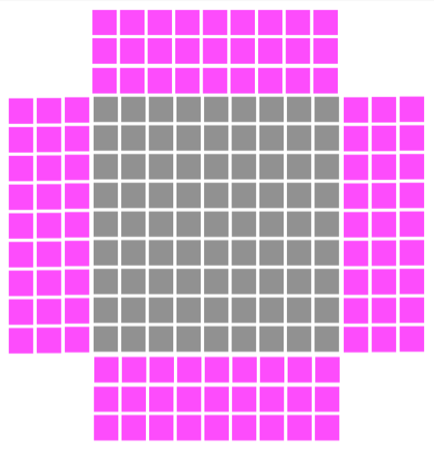
\includegraphics[width=0.3\textwidth]{figs/trigger/chunkyDonut}
    \label{fig:chunkystrips}
  }\\
  \caption{Various configurations of \TT strips around the Level-1 jet
  algorithm window used for donut subtraction}
  \label{fig:alldonutstrips}
\end{figure}

One of the main issues with the donut subtraction algorithm is this
sensitivity to fluctuations. It is mitigated by taking the median energy two strips
but can be further reduced by increasing the area covered by the
strips. The rings of \TTs can be extended to be three towers wide,
known as a \emph{chunky} donut and illustrated in
Fig.~\ref{fig:chunkystrips}. This is particularly effective in
reducing the fluctuations in the positions of \PU particles with
respect to the jet in consideration.

To confirm that the energy in the median two strips of the  chunky
donut is a good measure of the \PU in the event, it is plotted against
the number of interactions for a minimum bias \MC sample in
Fig.~\ref{fig:donut_nint}. There is a good correlation that appears to
pass through the origin, implying it is indeed a good measure of \PU. 
% note that the fact that it passes through the origin for ttbar
% indicates that the median strips reduce hard scatter contamination

\begin{figure}
	\begin{center}
		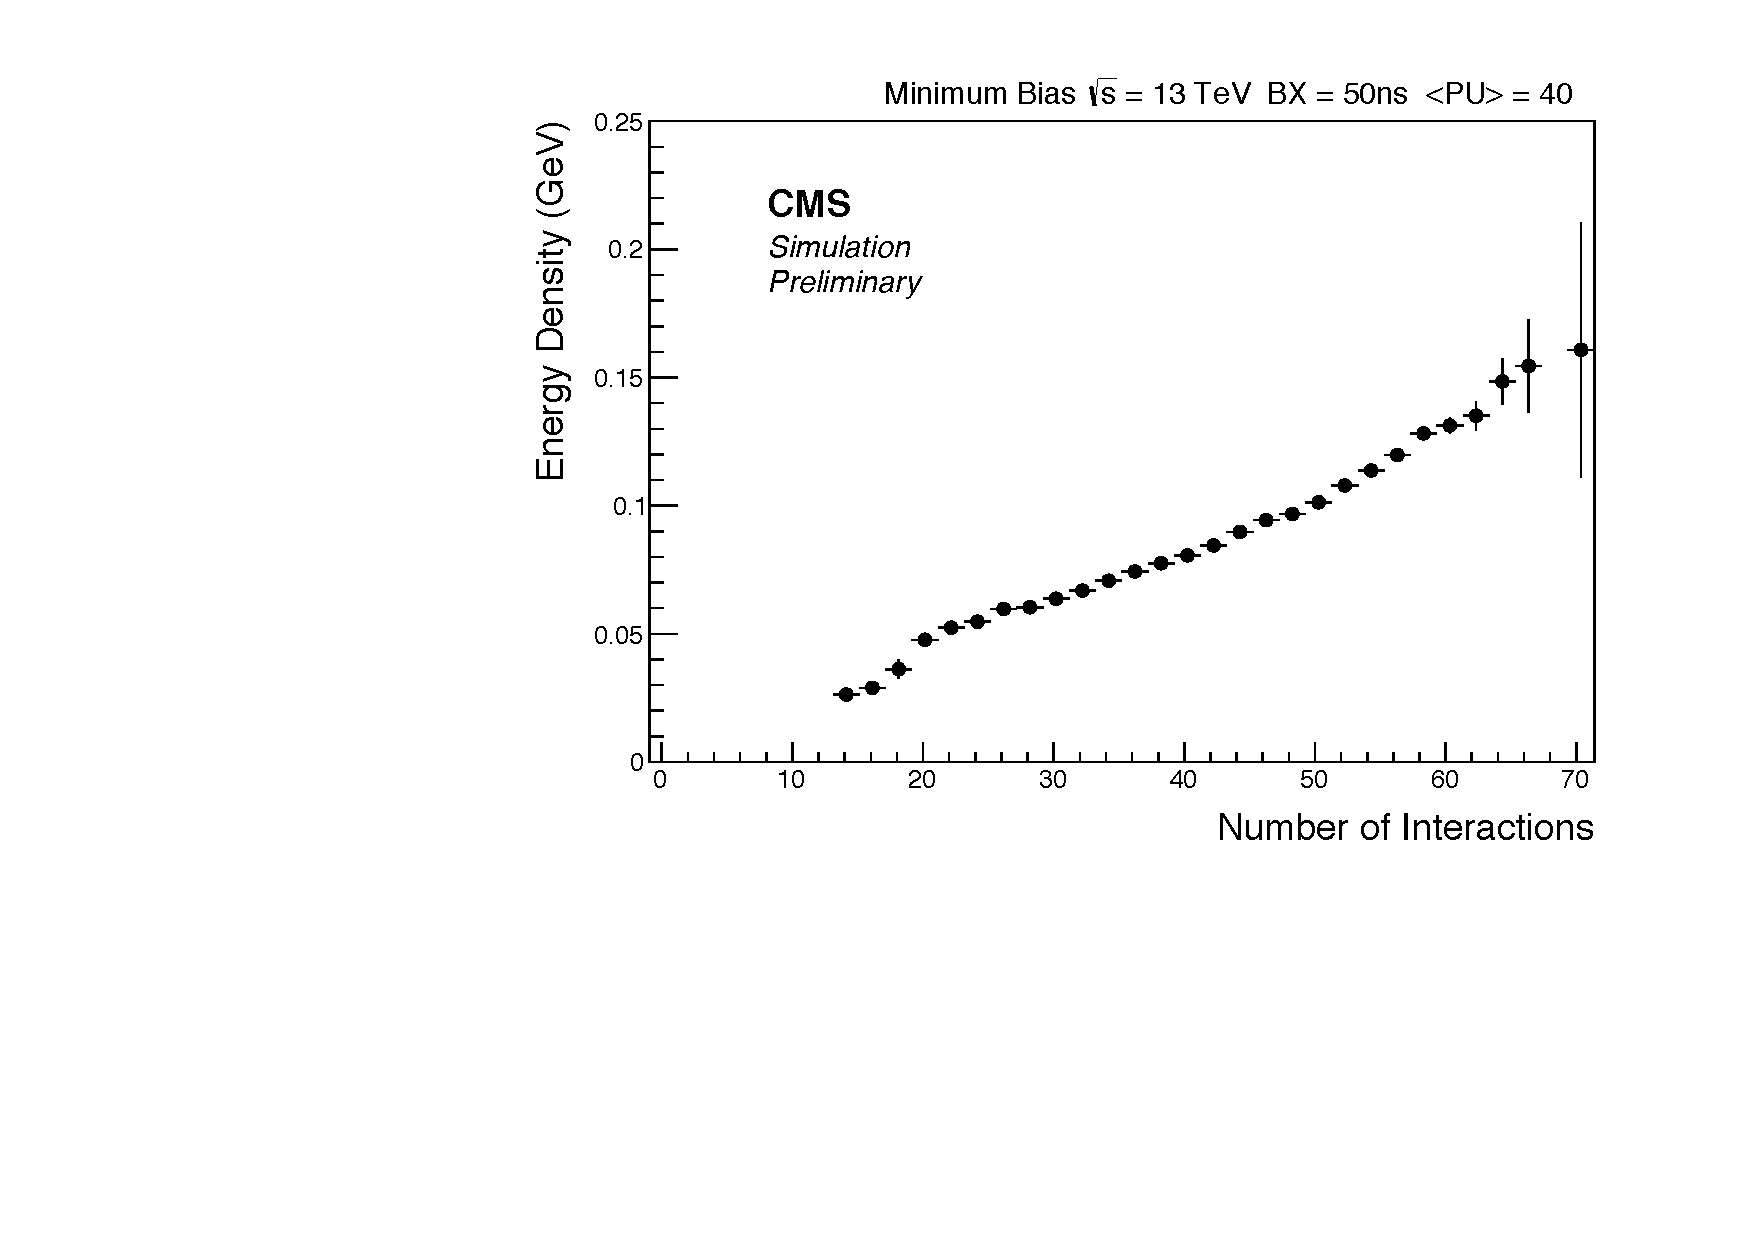
\includegraphics[width=0.8\linewidth]{figs/trigger/threestrips}
  \caption{The energy density in the median two $3\times 1$ \TT strips
  of a chunky donut around Level-1 jets in the \CMS calorimeters as a
  function of the number of simultaneous collisions. This is taken
  from minimum bias \MC simulation at 13~\tev with a 50~ns bunch
  crossing time}
	\label{fig:donut_nint}
	\end{center}
\end{figure}

In the implementation of the Level-1 jet finding algorithm in the
upgrade hardware, the \TTs that make up the donut are already
available in memory. This means donut subtraction has a very low
latency penalty. This presents a significant advantage over a global
\PUS. 

\subsection{Jet seed threshold and zero suppression}

Donut subtraction helps to remove the effects of \PU on the
reconstructed high energy jets, but is less successful at removing the
soft jets that are purely from \PU interactions. A simple way of
reducing the number of soft jets is by introducing an energy threshold
on the \TT that can form a jet. The \TT that is considered for a jet
candidate in the algorithm outlined in
Section~\ref{sec:stage2_jetalgo} is required to be above a certain
energy, known as the seed threshold. This is very easy to implement in
hardware, and has the potential to save latency as it reduces the
number of jets that need to be made. A disadvantage is that it can
kill soft jets that originate from a primary vertex. It also does not
account for any $\eta$ dependence. For the studies in
Sec.~\ref{sec:jet_algo_performance} a seed of $2.5$~GeV was
chosen as a benchmark that appeared to kill PU jets without removing
jets above 10~GeV from a zero PU $t\bar{t}$ \MC simulation. This is
demonstrated in Fig.~\ref{fig:noPUSeedTTbar}. As the Level-1 hardware
measures energy in units corresponding to 0.5~\gev (\emph{L1-units}),
this is denoted as \emph{Seed 5}. 

\begin{figure}
	\begin{center}
		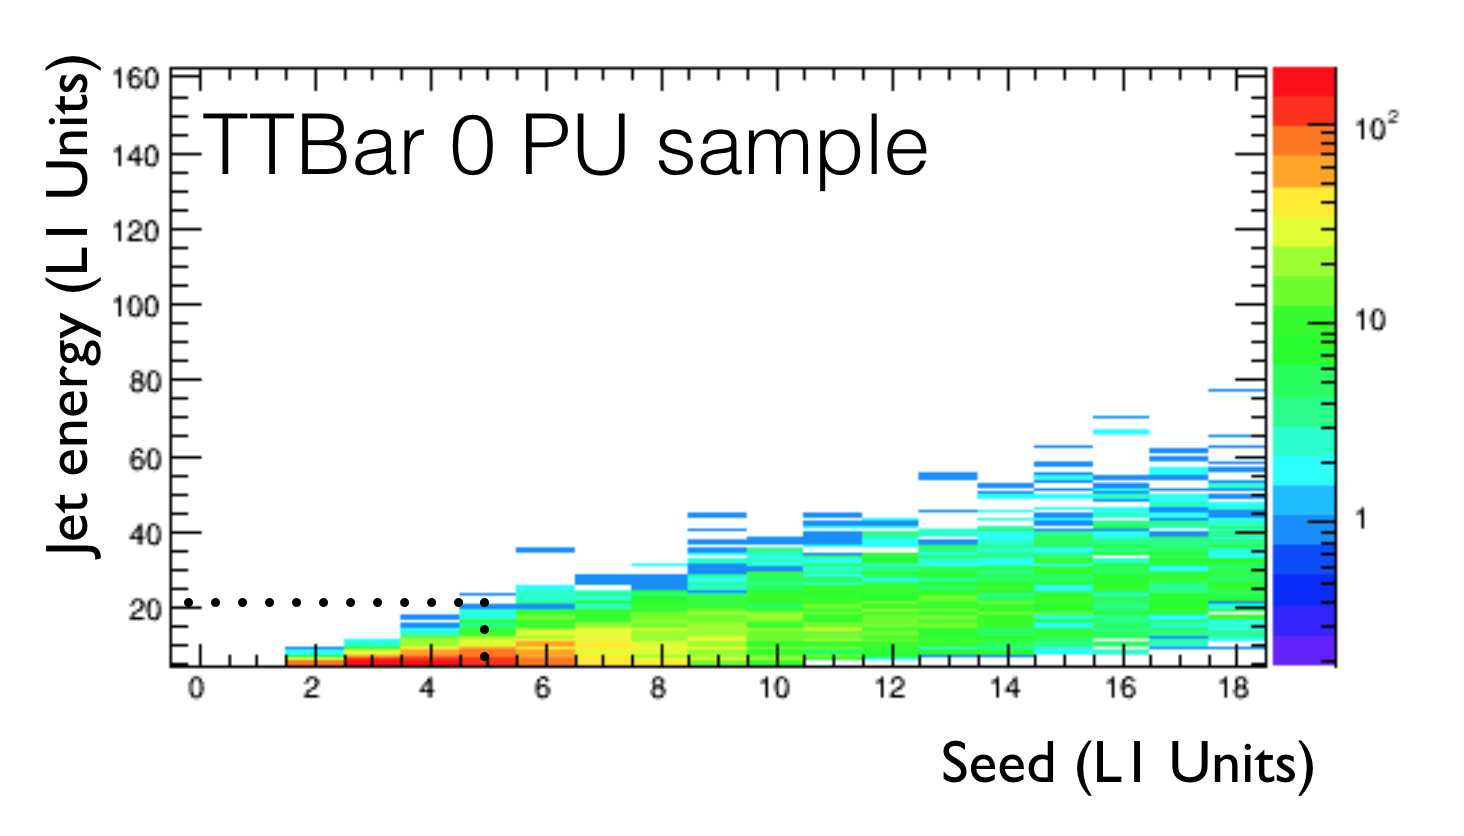
\includegraphics[width=0.8\linewidth]{figs/trigger/noPUSeedTTbar}
  \caption{The Level-1 jet energy vs seed threshold for a simulated
  sample of top quark pair production events with no overlaid \PU. The
  units of energy are \emph{L1-units}, which correspond to 0.5~\gev
  each. A seed threshold of 2.5~\gev only removes up to 10~\gev jets
  from the hard scatter.}
	\label{fig:noPUSeedTTbar}
	\end{center}
\end{figure}

To remove the effects of noise on the Level-1 trigger inputs, a
\emph{zero-suppression} is performed that requires \TTs to have an
energy above 0.5~\gev before they are considered to have any energy at
all. As \PU is expected to result in much smaller energy deposits than
interesting physics processes, the effect of increasing the energy
that is suppressed to zero when building the jets also acts as a form
of \PUS. This form of \PUS is considered in
Sec.~\ref{sec:jet_algo_performance} and is named Tower Suppression
(TSup). Despite being very easy to implement in hardware this
algorithm does not adapt well to different \PU conditions and can
reduce the energy resolution of the jets.

\section{Level-1 jet energy calibration}
\label{sec:l1jec}

To obtain Level-1 jets that correspond as closely as possible to the
true physics objects that they represent, their energy must be
corrected. The
varying response of the \HCAL and \ECAL as a function of jet \pT and
\eta necessitates a calibration that depends on these variables.  The
need for calibration in the Level-1 trigger is exacerbated by the
coarse level of information available compared to that in offline
reconstruction.

The calibration is performed using QCD dijet \MC simulation with an
average \PU of 40. Samples were generated with a range of generator
scales from 10 to 600~\gev. These energies characterise the \pT of the
leading jet and ensure a wide range of jet energies are available.
From this sample, \emph{generator jets} are clustered from
the truth-level particles, the final result of the procedure
described in Sec.~\ref{sec:mc_reco}. Clustering is performed with the
anti-$k_T$ algorithm with $R=0.4$, after removing any muon and
neutrino particles. This ensures that the Level-1 jets are just
calibrated based on the particles that are deposited in the
calorimeters. The Level-1 jet algorithm is performed on the simulated
Level-1
trigger calorimeter inputs. Each Level-1 jet is matched to the
generator jet that is closest in $\Delta
R=\sqrt{(\Delta\eta)^2+(\Delta\phi)^2}$ to the central \TT of the jet.
If a generator level jet cannot be found within $\Delta R<0.3$, the
Level-1 jet in question is ignored. The \pT of the Level-1 jet
(L1~\pT) after \PUS is compared to the \pT of the generator jet
(GEN~\pT) and the response is defined as the ratio of these two
quantities, L1~$\pT/$GEN~\pT.
% from Kristian via Adinda about what the PT hat is:
% The is the Pt scale of the "internal quark line" in the Feynman
% diagram for QCD multi-jet production.
% It sets a typical scale of the highest Pt jet, but in most events
% there will be softer jets from parton showers in addition.

The distribution of the response is plotted in bins of generator jet
\pT for each of the matched jet pairs. A Gaussian function is fit to the
response to obtain an estimate for the mean response and standard
deviation in a $2~\gev$ bin of generator jet \pT. The response is
inverted to provide a corrective scale factor for the Level-1 jets. It
is fit to a calibration function as a function of the L1~\pT in eight
bins of \eta, up to $|\eta|<3.0$ \cite{l1triggernote2012}. The
function has the form:
\begin{equation}
\langle \pT^{L1}/\pT^{GEN} \rangle ^{-1} =
(p_0 + \frac{p_1}{(\log\pT^{L1})+p_2} + p_3 \exp(-p_4(\log
\pT^{L1}-p_5)^2)),
\end{equation}
where $p_n$ are free parameters to be found with a $\chi^2$
minimisation fit, $\pT^{L1}$ is the Level-1 jet \pT and $\pT^{GEN}$ is
the matched generator jet \pT. This parameterisation provides a
multiplicative correction that can be applied to Level-1 jets as they
are produced online where their original \pT, $\pT^{raw}$, can be
corrected to $\pT^{corr}$ via:
\begin{equation}
 \pT^{corr}=\pT^{raw} \langle \pT^{L1}/\pT^{GEN} \rangle ^{-1}. 
\end{equation}
The inverse response as a function of Level-1 jet \pT for Level-1 jets
produced with chunky donut subtraction and a central seed of 2.5~\gev
are shown in Fig.~\ref{fig:calibFunctions}.

\begin{figure}
  \centering
  \subfloat[$0.00<\eta<0.75$]{
    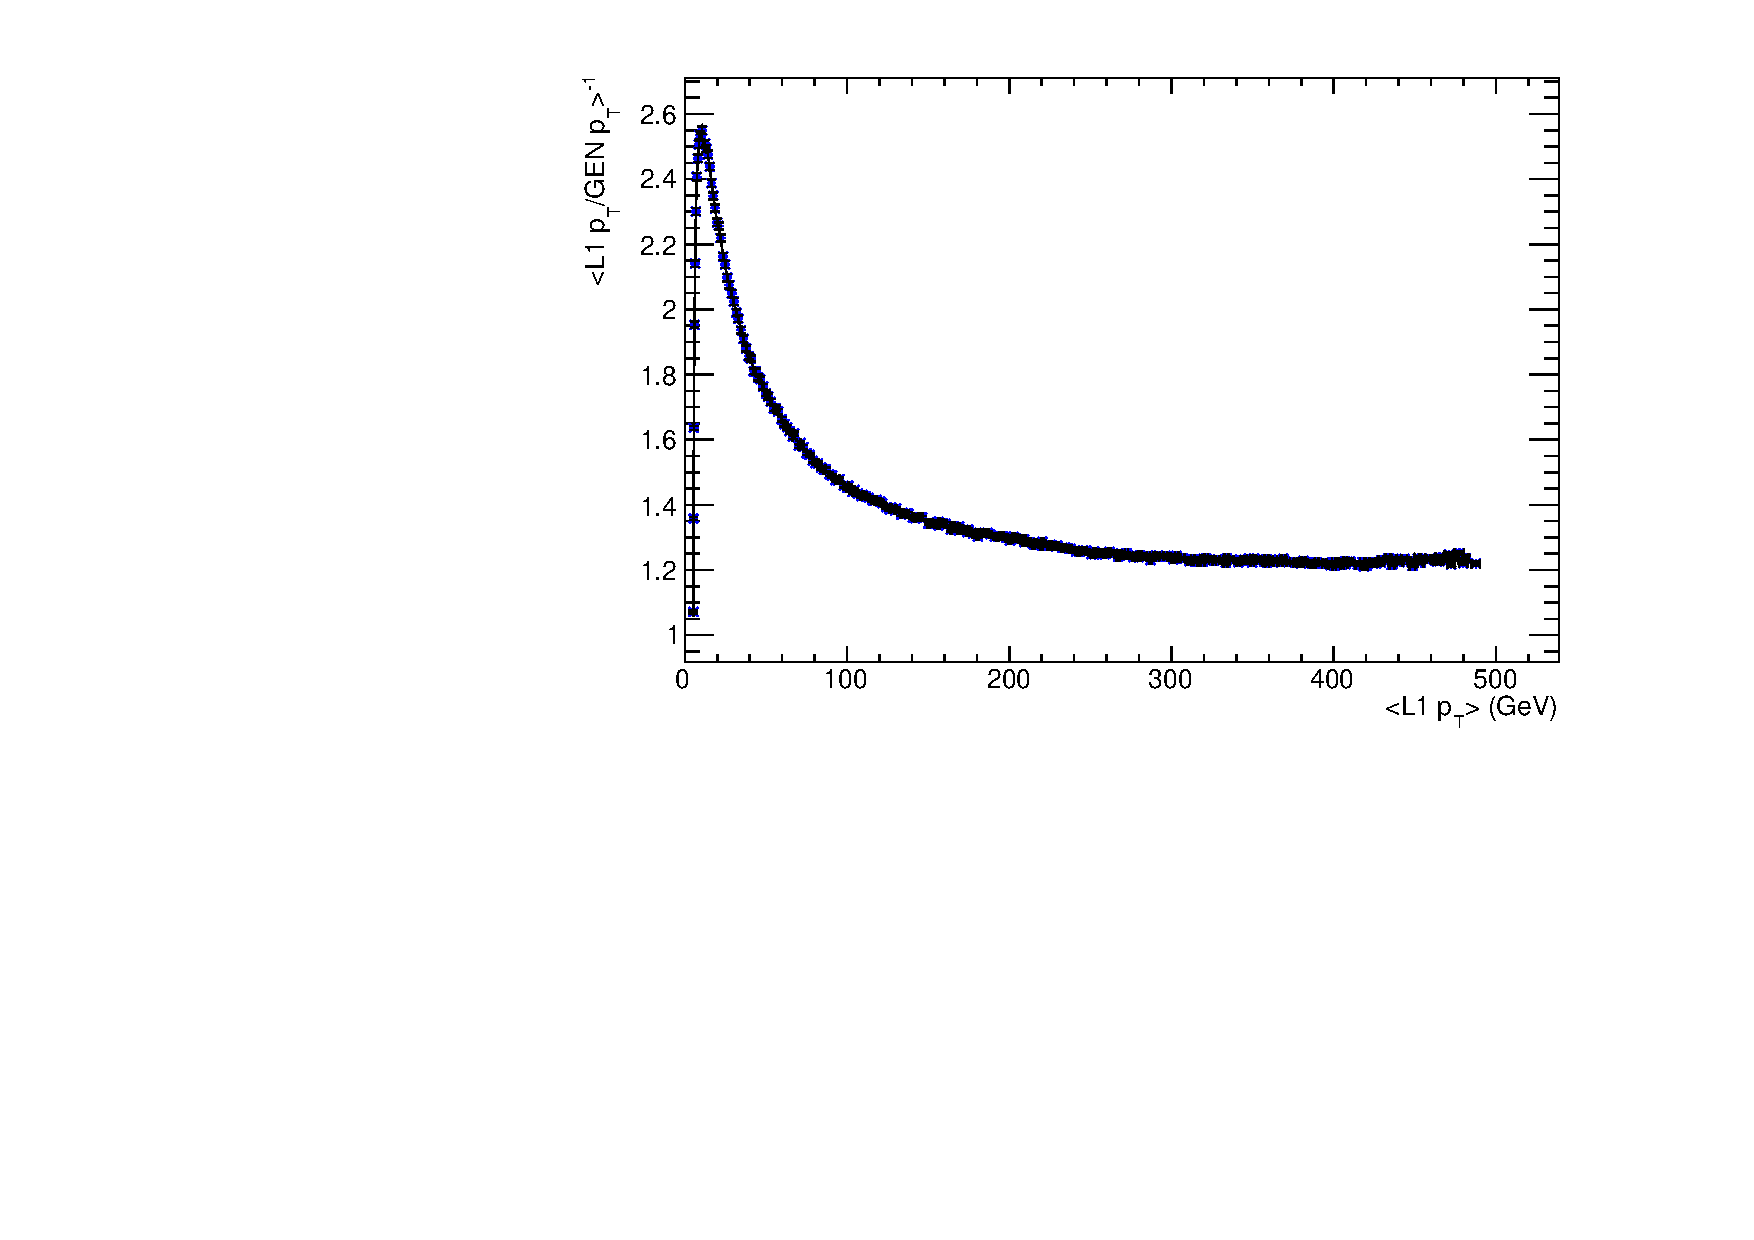
\includegraphics[width=0.5\textwidth]{figs/trigger/p1}
  }~ 
  \subfloat[$0.75<\eta<1.50$]{
    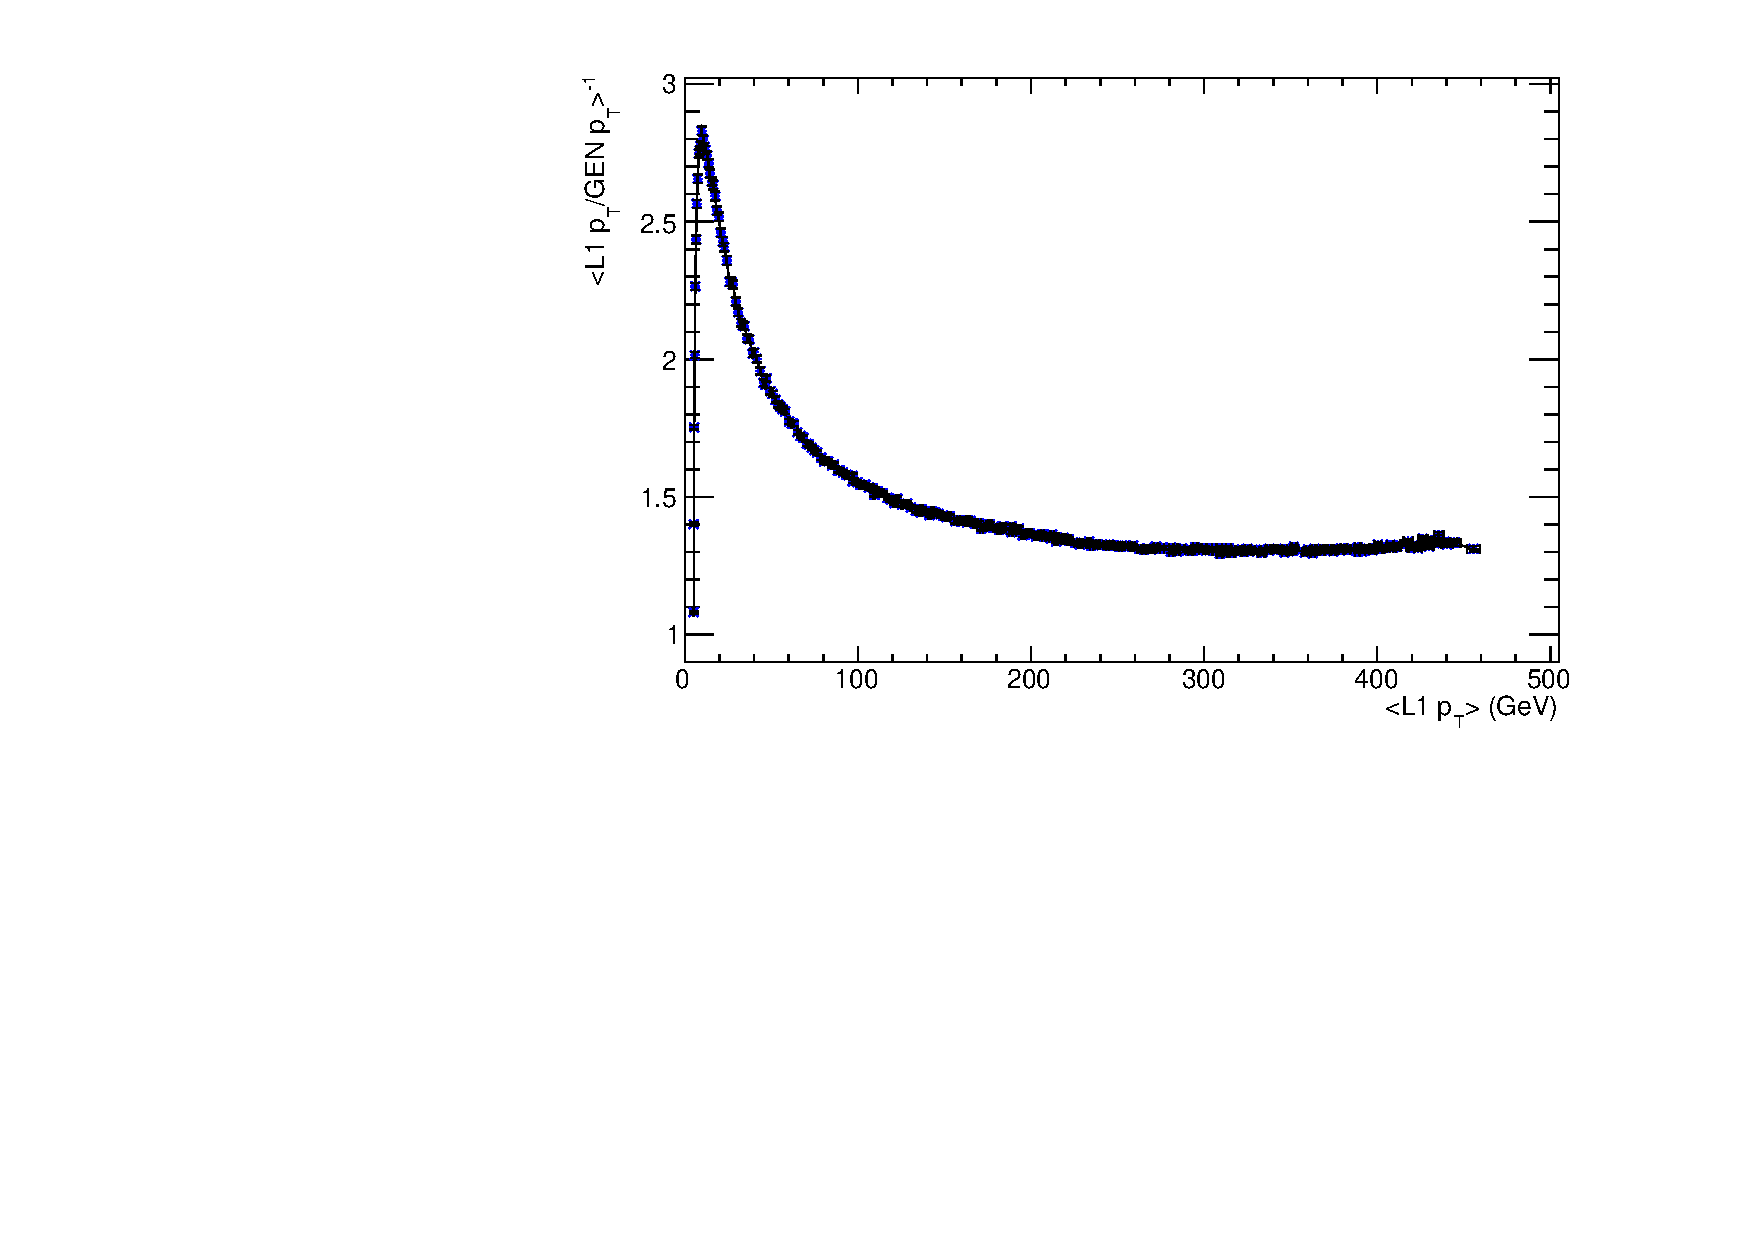
\includegraphics[width=0.5\textwidth]{figs/trigger/p2}
  }\\
  \subfloat[$1.50<\eta<2.25$]{
    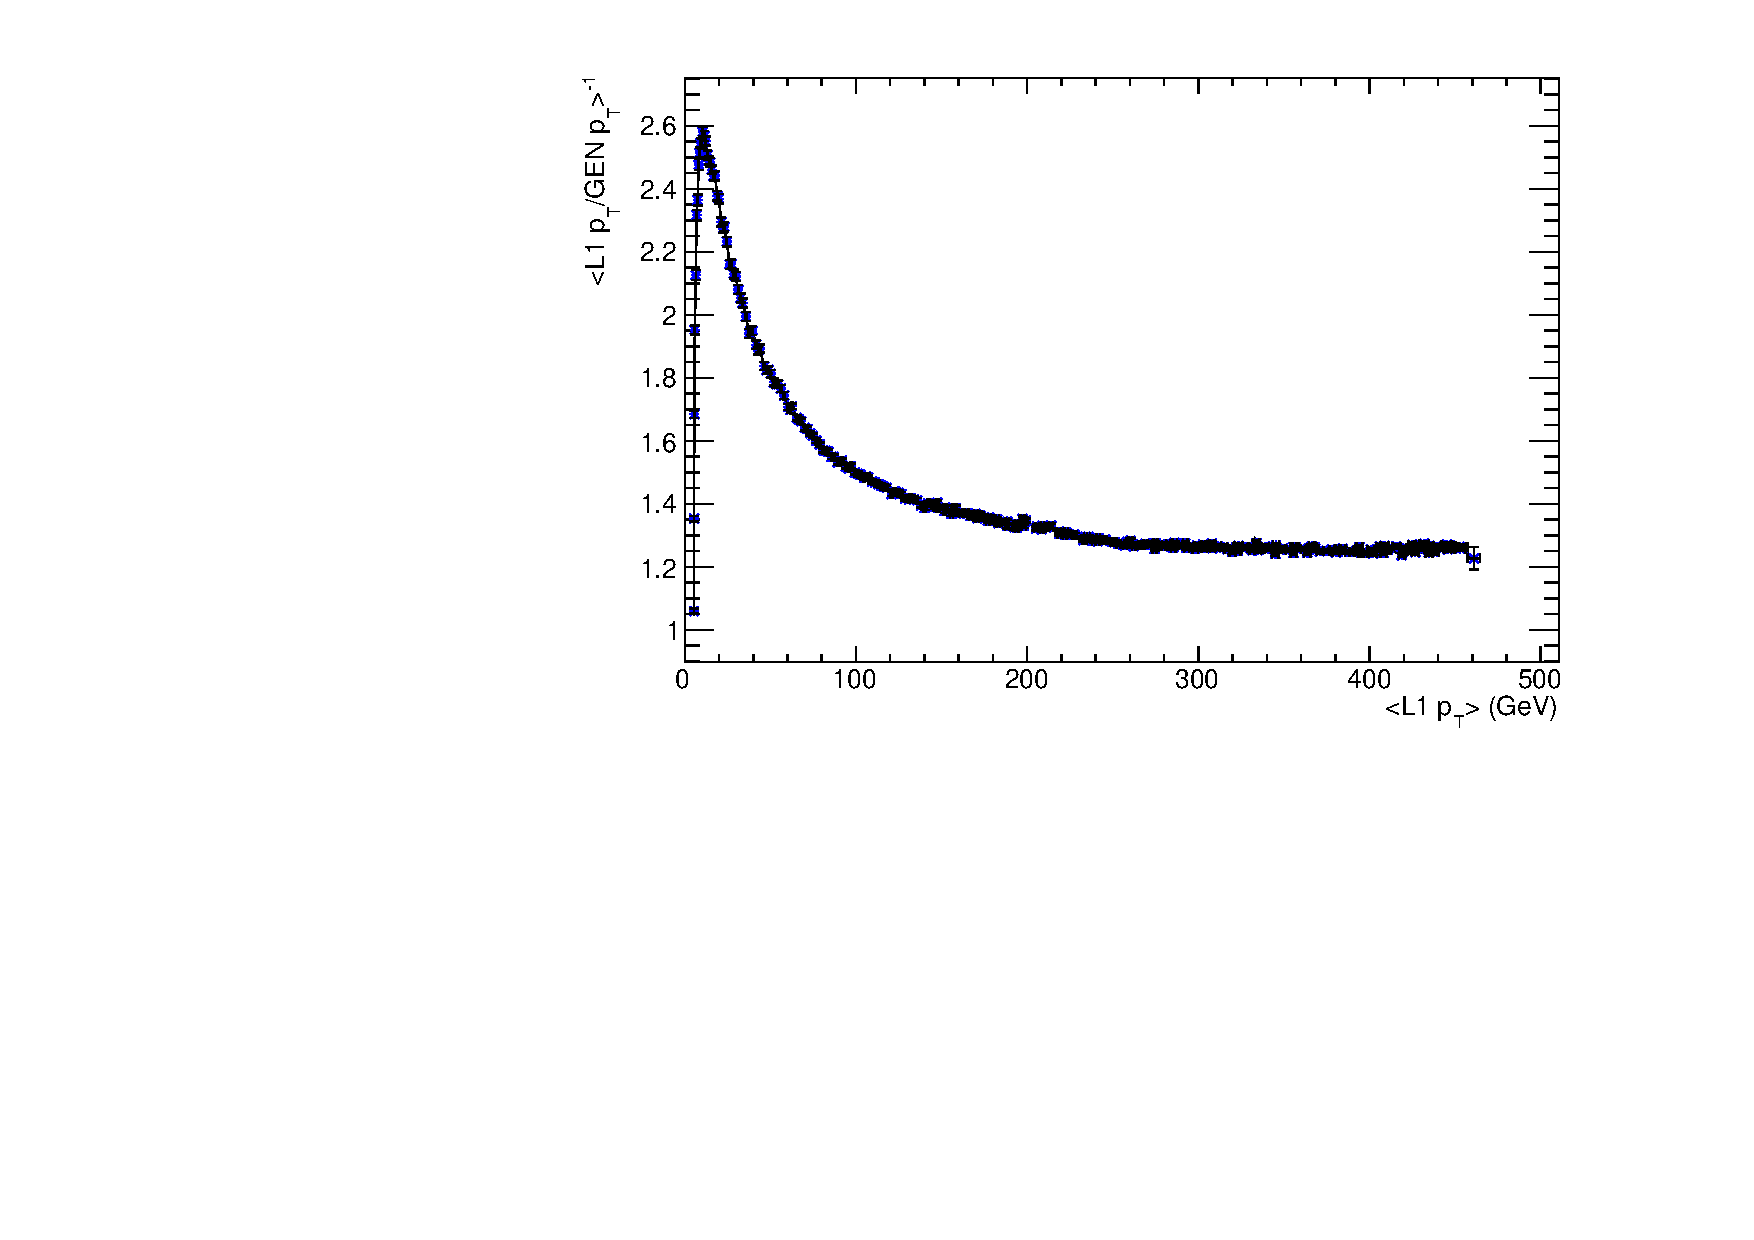
\includegraphics[width=0.5\textwidth]{figs/trigger/p3}
  }~ 
  \subfloat[$2.25<\eta<3.00$]{
    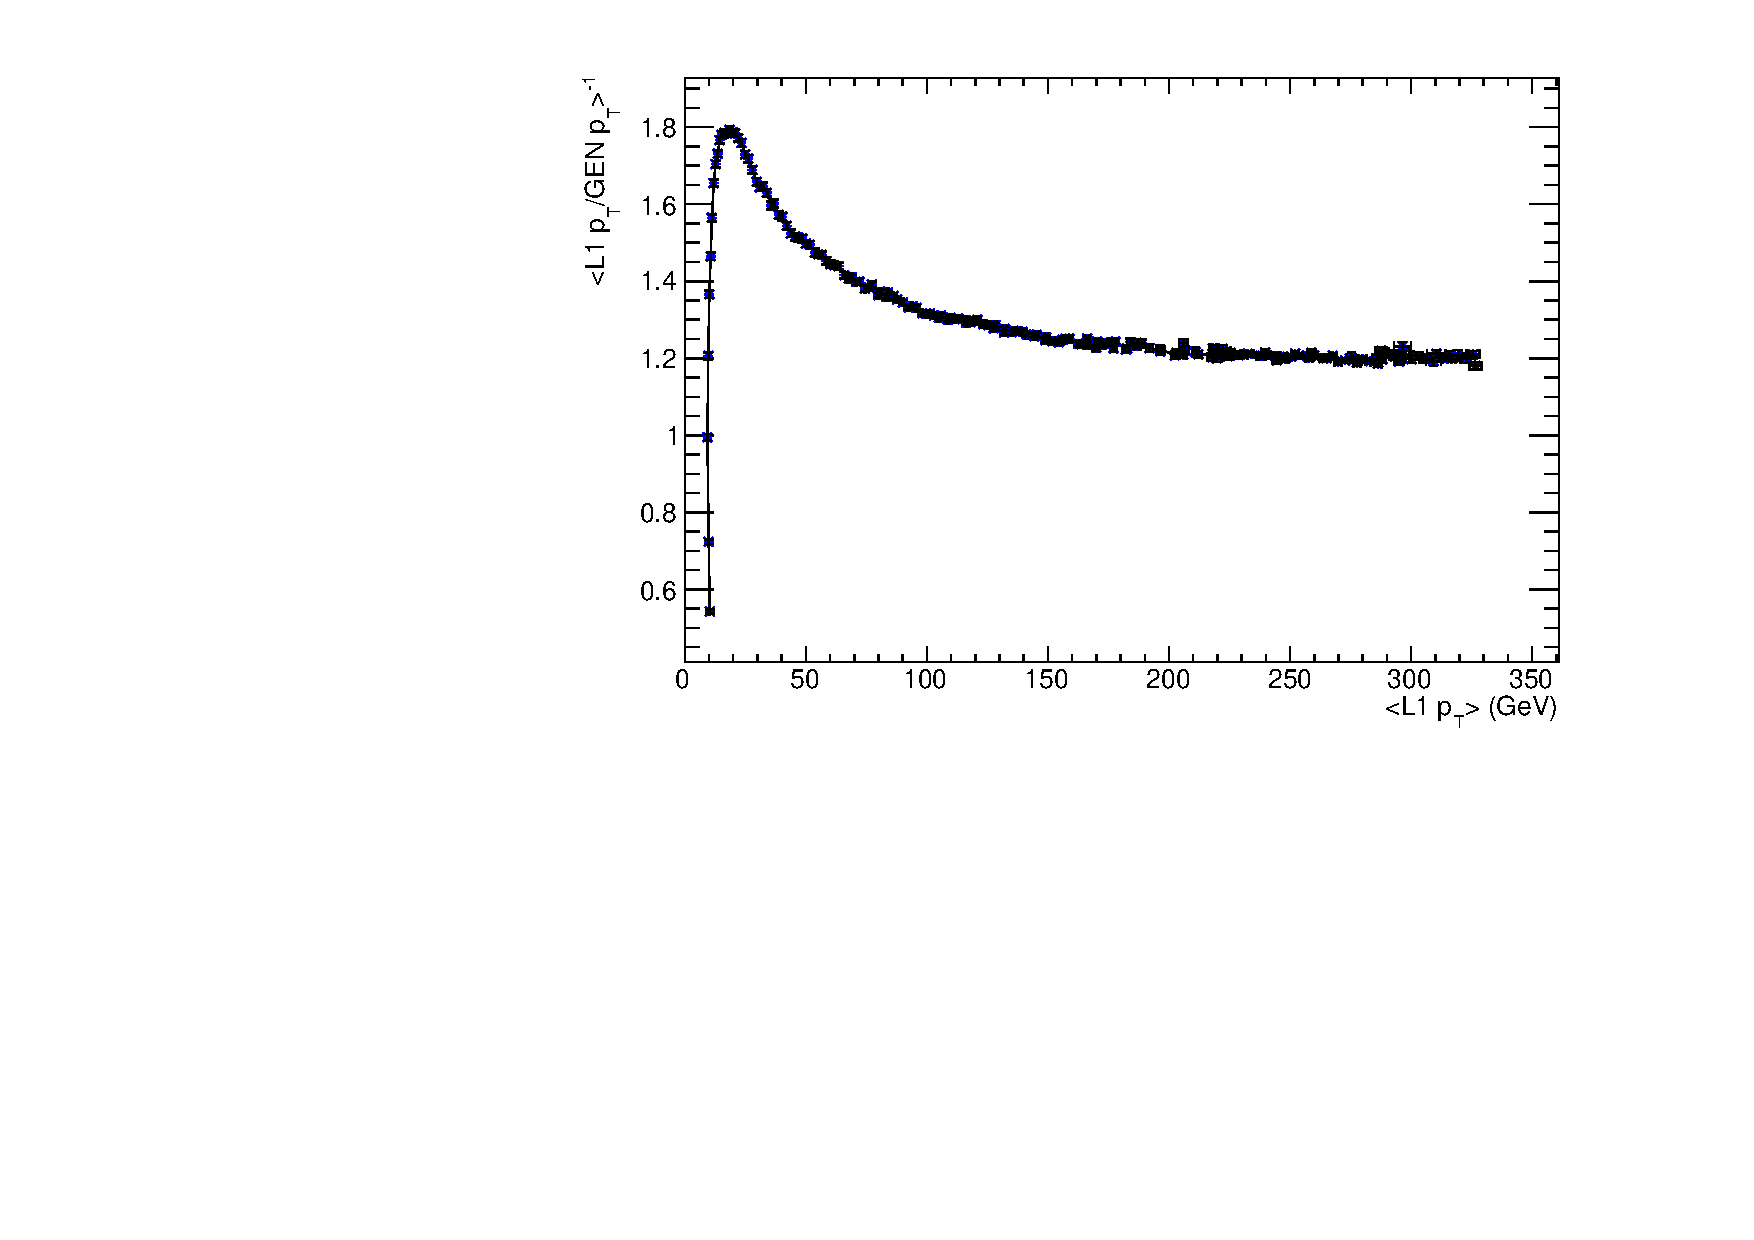
\includegraphics[width=0.5\textwidth]{figs/trigger/p4}
  }\\
  \subfloat[$-0.75<\eta<0.00$]{
    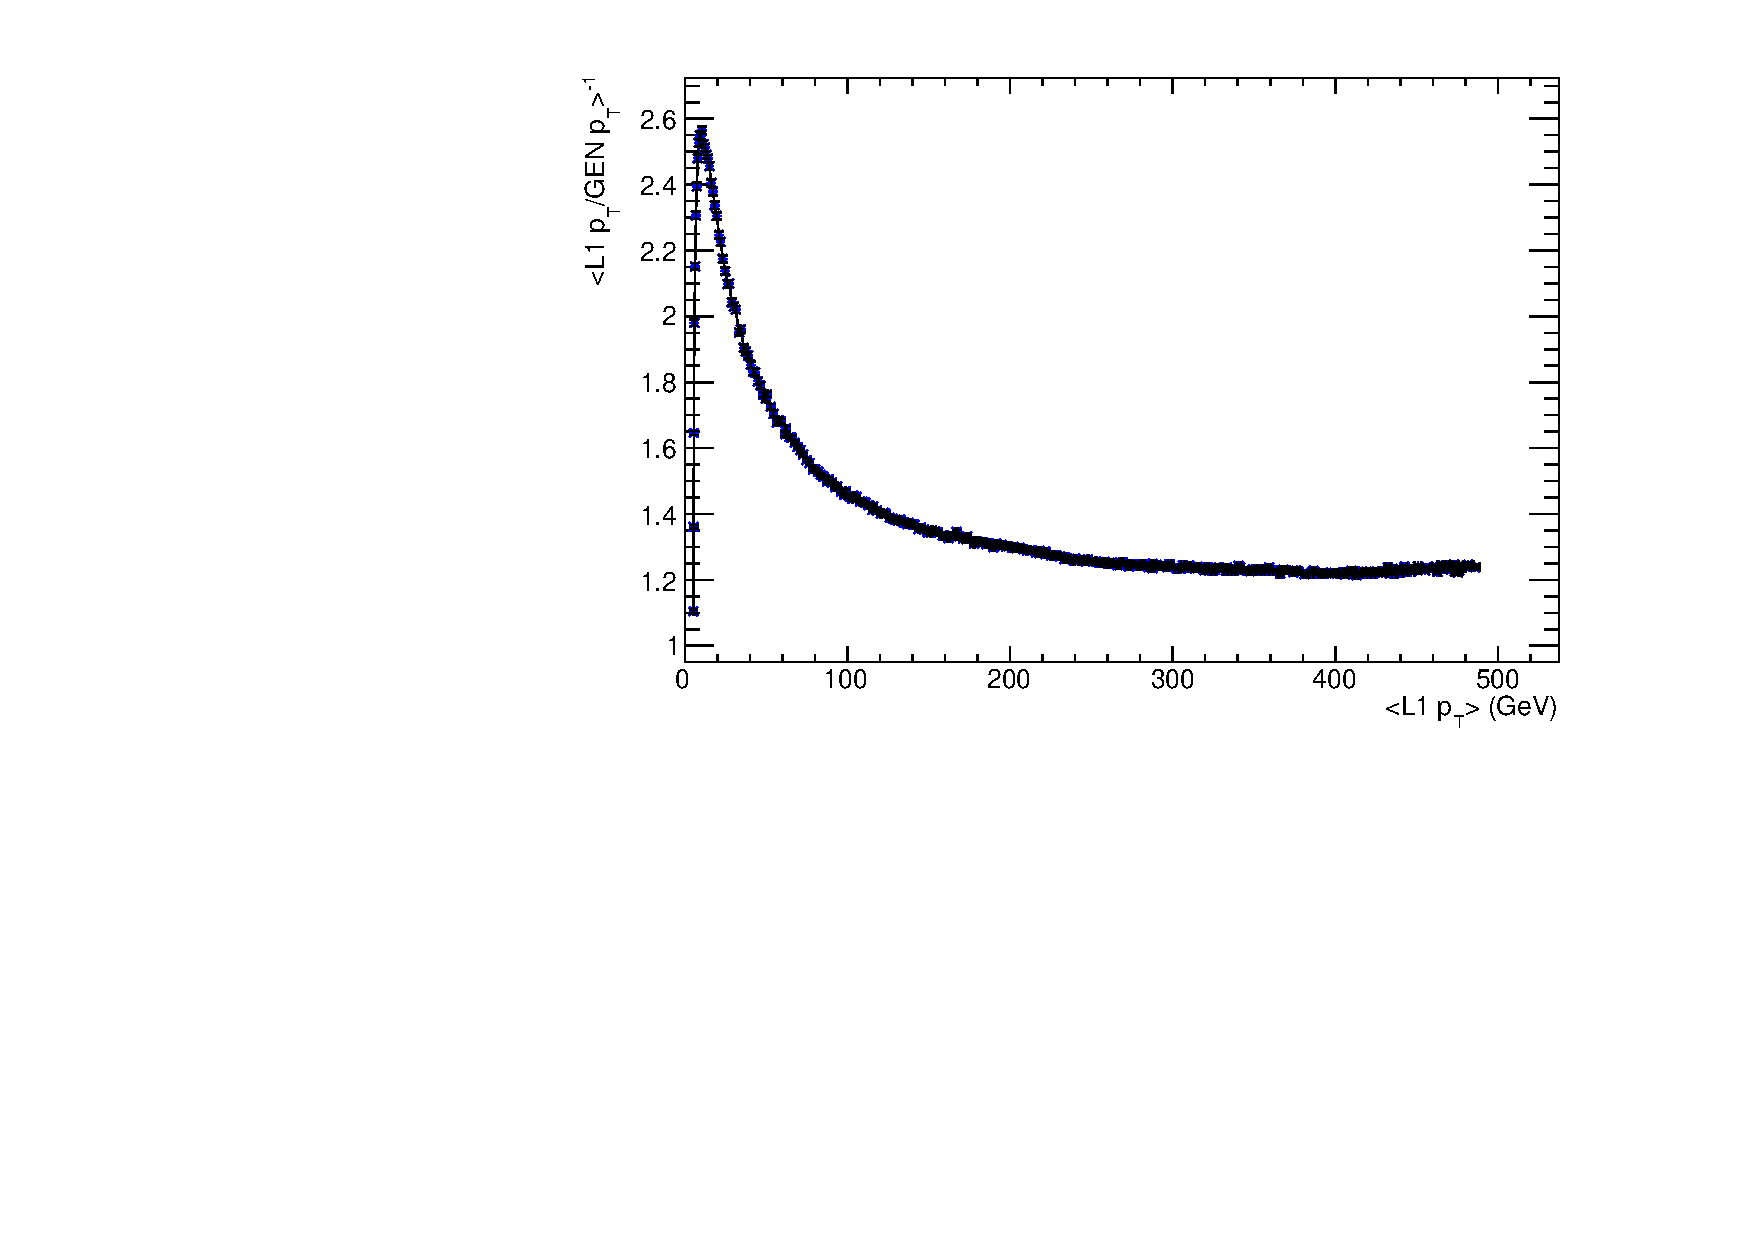
\includegraphics[width=0.5\textwidth]{figs/trigger/m1}
  }~ 
  \subfloat[$-1.50<\eta<-0.75$]{
    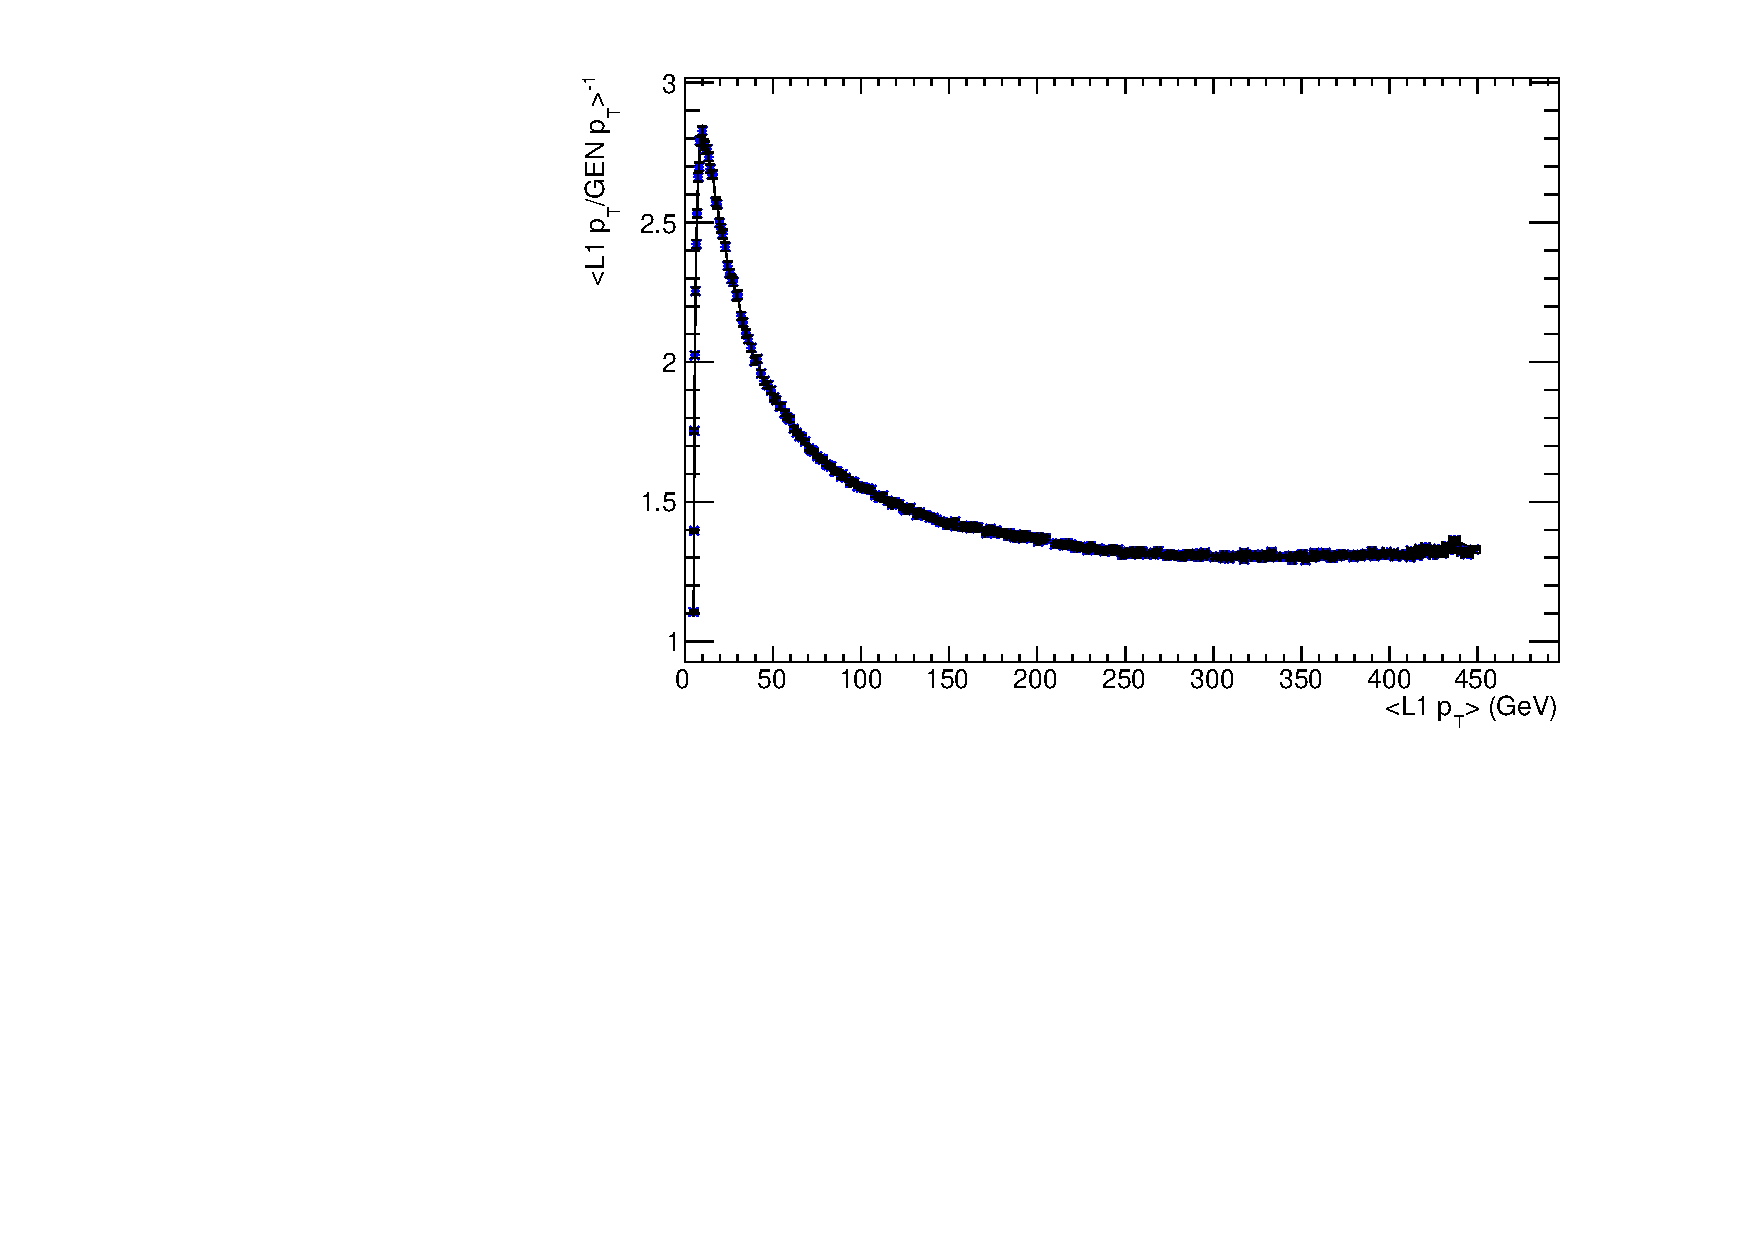
\includegraphics[width=0.5\textwidth]{figs/trigger/m2}
  }\\
  \subfloat[$-2.25<\eta<-1.50$]{
    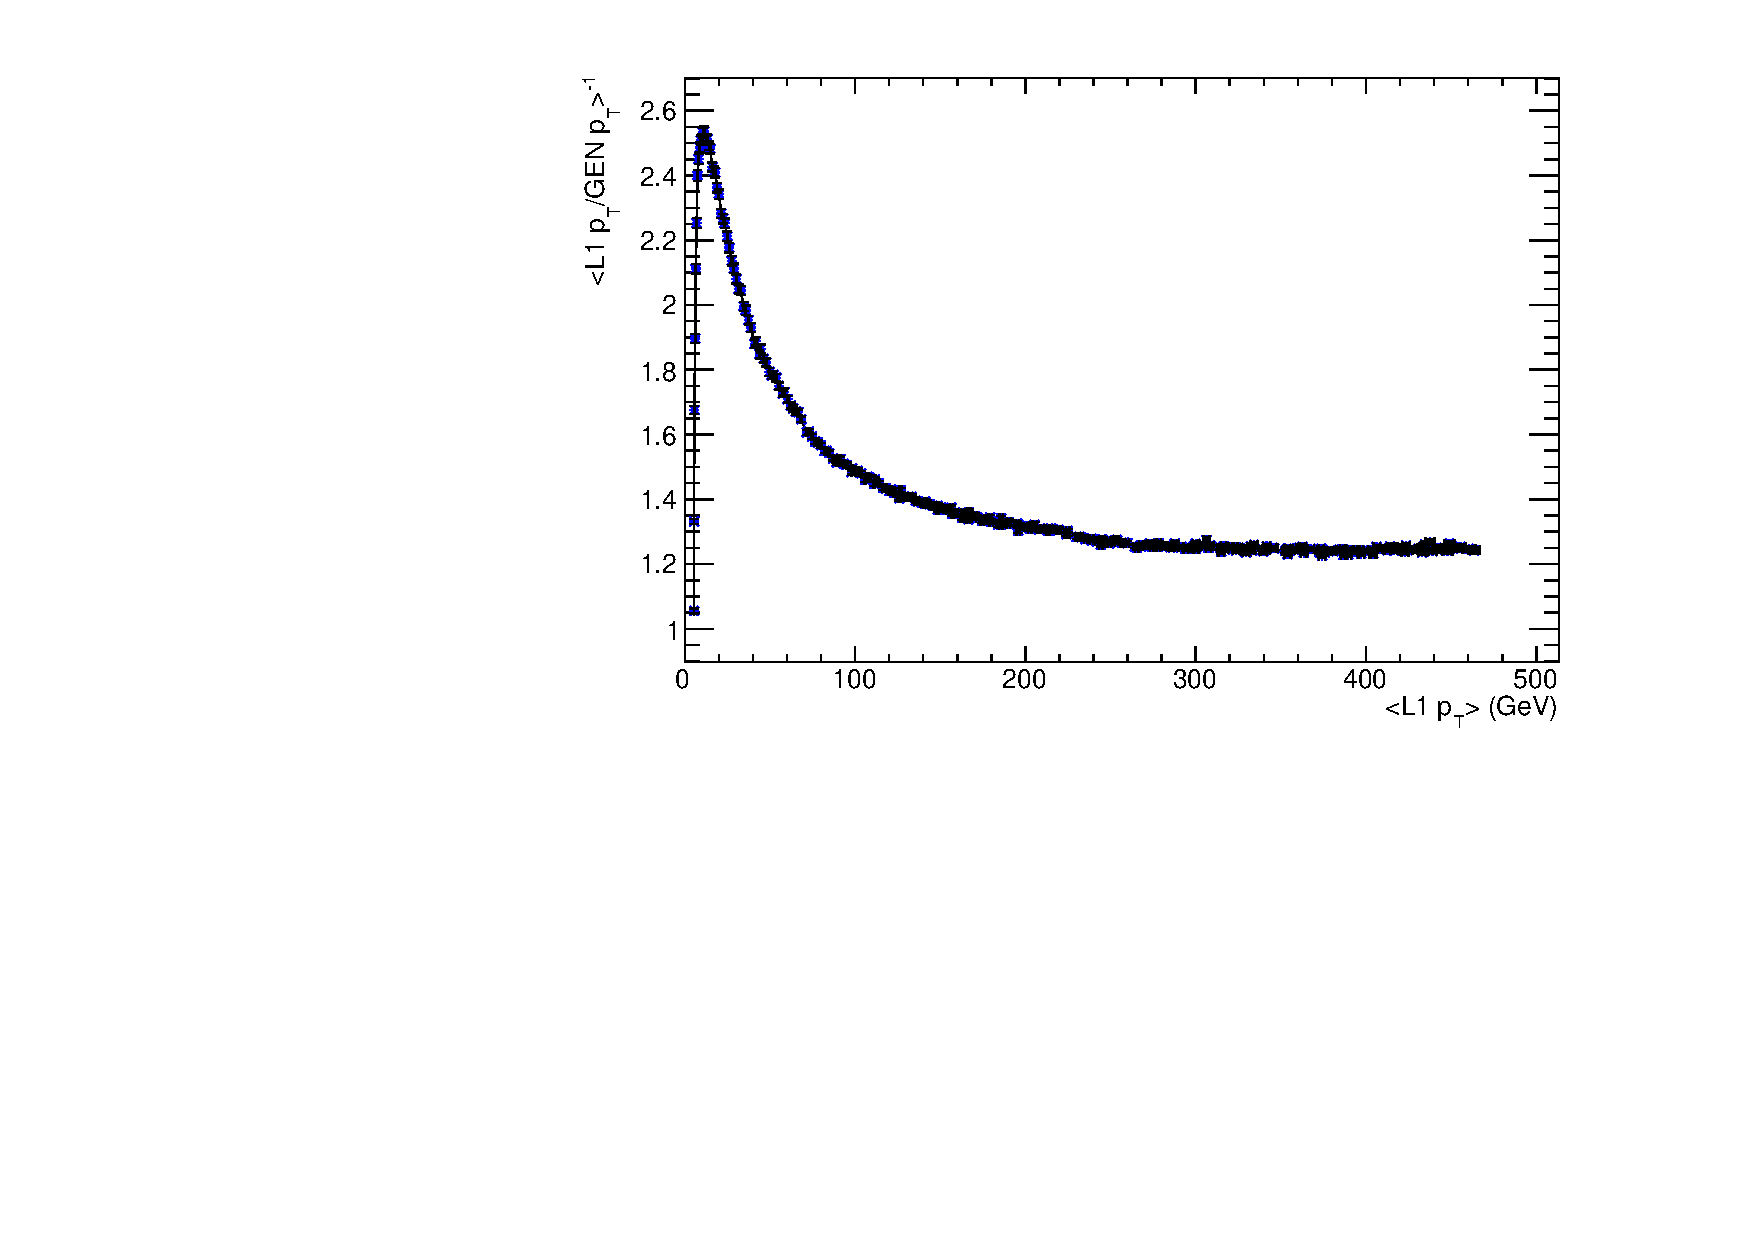
\includegraphics[width=0.5\textwidth]{figs/trigger/m3}
  }~ 
  \subfloat[$-3.00<\eta<-2.25$]{
    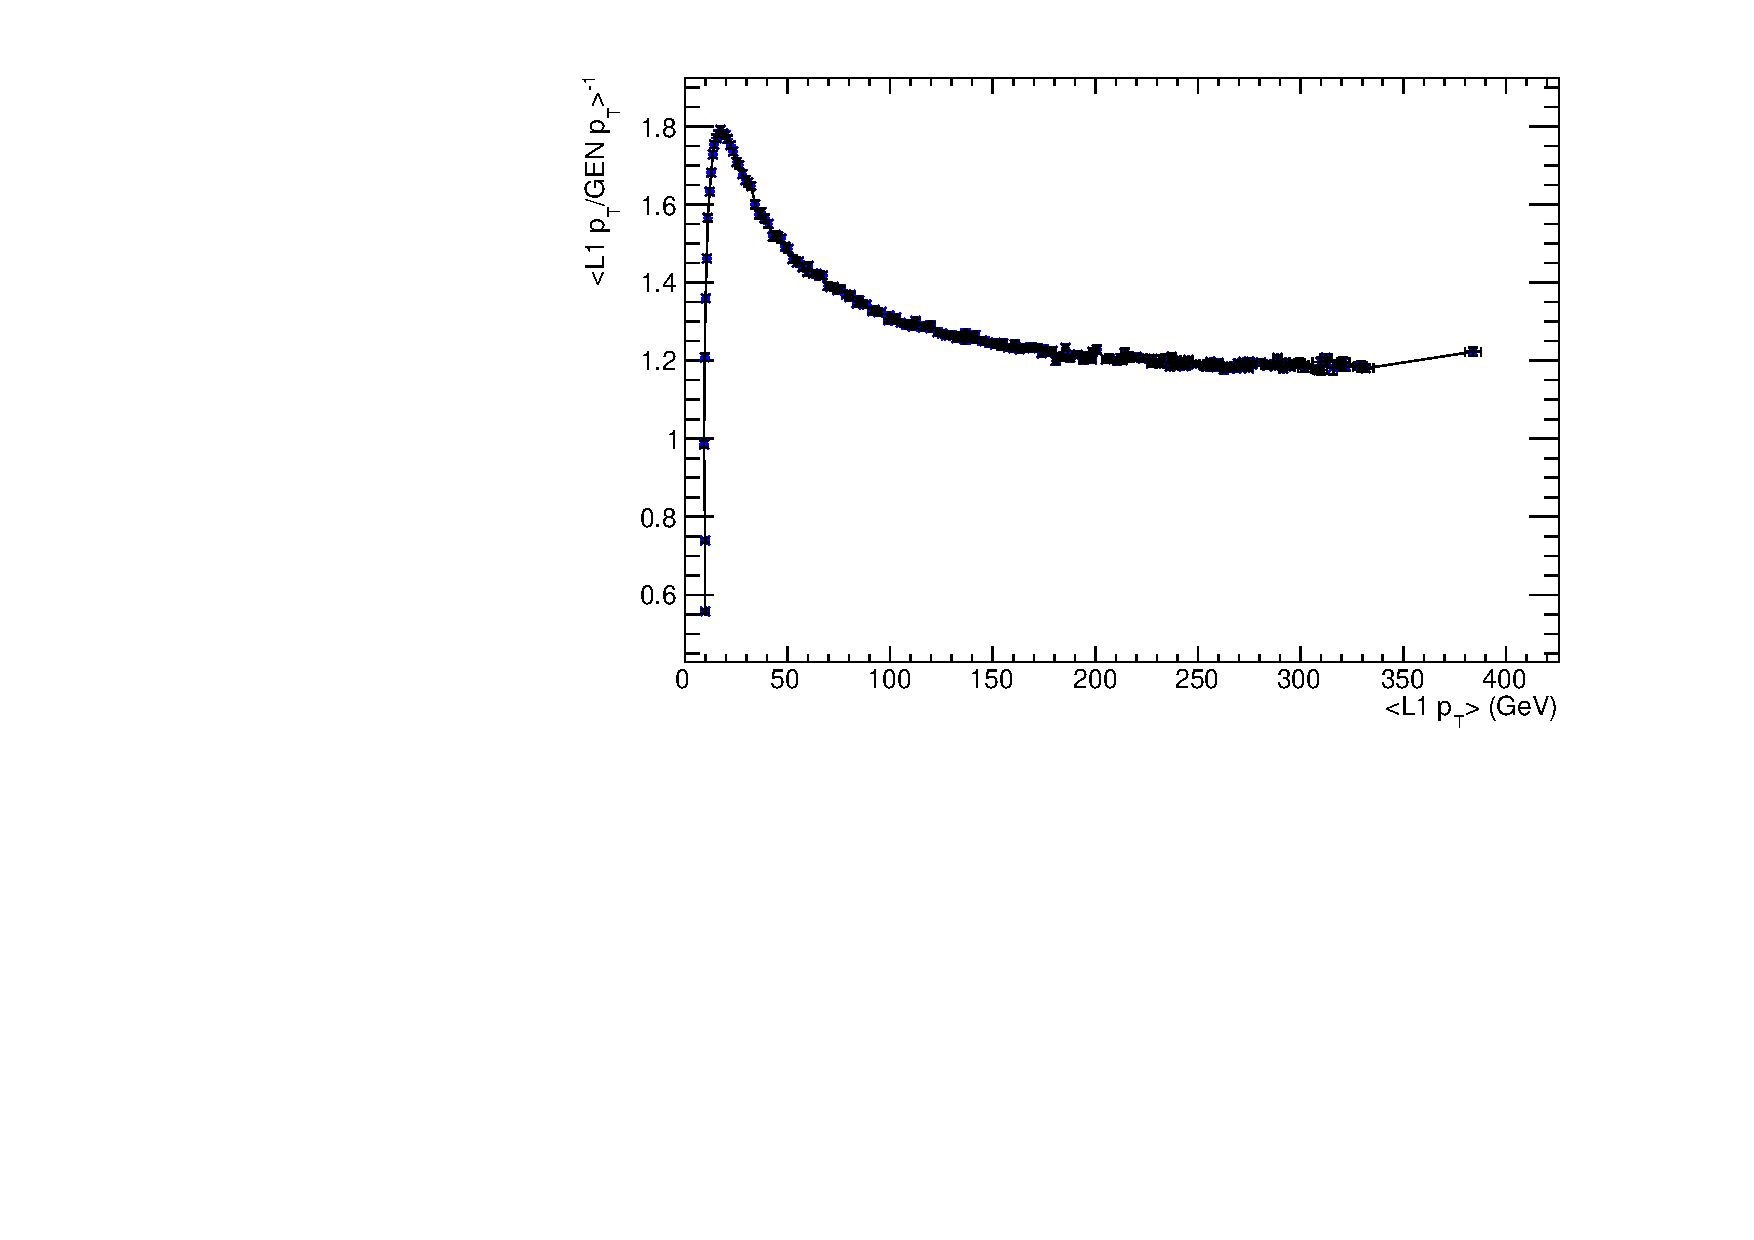
\includegraphics[width=0.5\textwidth]{figs/trigger/m4}
  }
  \caption{Calibration fits across all \eta ranges as a function of
  Level-1 jet \pT}
  \label{fig:calibFunctions}
\end{figure}

To test the calibration procedure a closure test is performed by
applying the calibration function to the simulation that was
used to derive it. The mean response as a function of generator jet
\pT in the range  $|\eta|<1.4$ is shown in
Fig.~\ref{fig:calibclosure} as an example. The
calibration procedure produces a flat response at unity for jets with
$\pT>50~\gev$. Below this value the matching procedure starts to
break-down, as low \pT Level-1 jets are less likely to be matched to a
corresponding generator jet. The Level-1 jets that are matched to a
generator jet are more likely to have a higher value of $\pT$, as
higher $\pT$ jets are more likely to be identified. This skews the
response upwards as the closure test approaches low values of $\pT$.
From observing a series of such closure tests it was concluded that it
was reasonable to consider Level-1 jets with a $\pT>20~\gev$, as in
this case the corrected response was reasonably compatible with unity.

\begin{figure}
	\begin{center}
		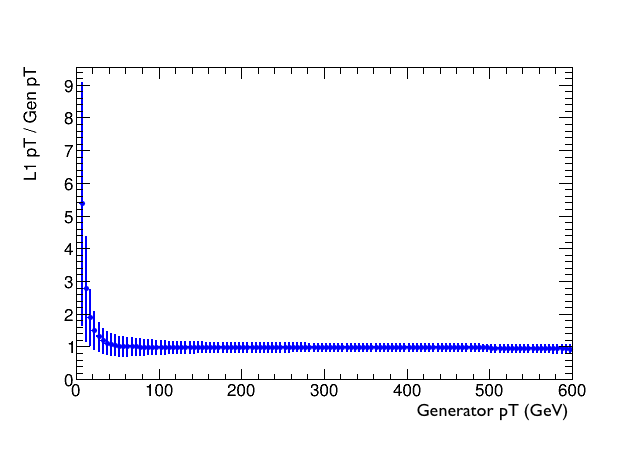
\includegraphics[width=0.8\linewidth]{figs/trigger/calibClosure_s5_donut}
  \caption{Closure test of the calibration procedure, checking the
  response as a function of generator jet \pT in the $|\eta|<1.4$ range.}
  \label{fig:calibclosure}
	\end{center}
\end{figure}

In future upgrades of the \LHC it is proposed to increase the \PU to
$\sim 140$. This will provide a much higher instantaneous luminosity,
but presents a significant challenge for reconstruction. To help
inform this upgrade, the Level-1 jets were produced and calibrated on a
sample with an average \PU of 140. The resulting jet response as a
function of generator jet \pT and Level-1 jet \eta can be seen in
Fig.~\ref{fig:pu140calibclosure}. The calibration was performed on
jets with a seed of 2.5~\gev and chunky donut subtraction. The
response is within $10\%$ of unity up to $|\eta|<2.5$ and for Level-1
jets with $\pT>50~\gev$. This suggests that the calibration and \PUS
procedure scales reasonably well with the number of \PU interactions.

\begin{figure}
	\begin{center}
		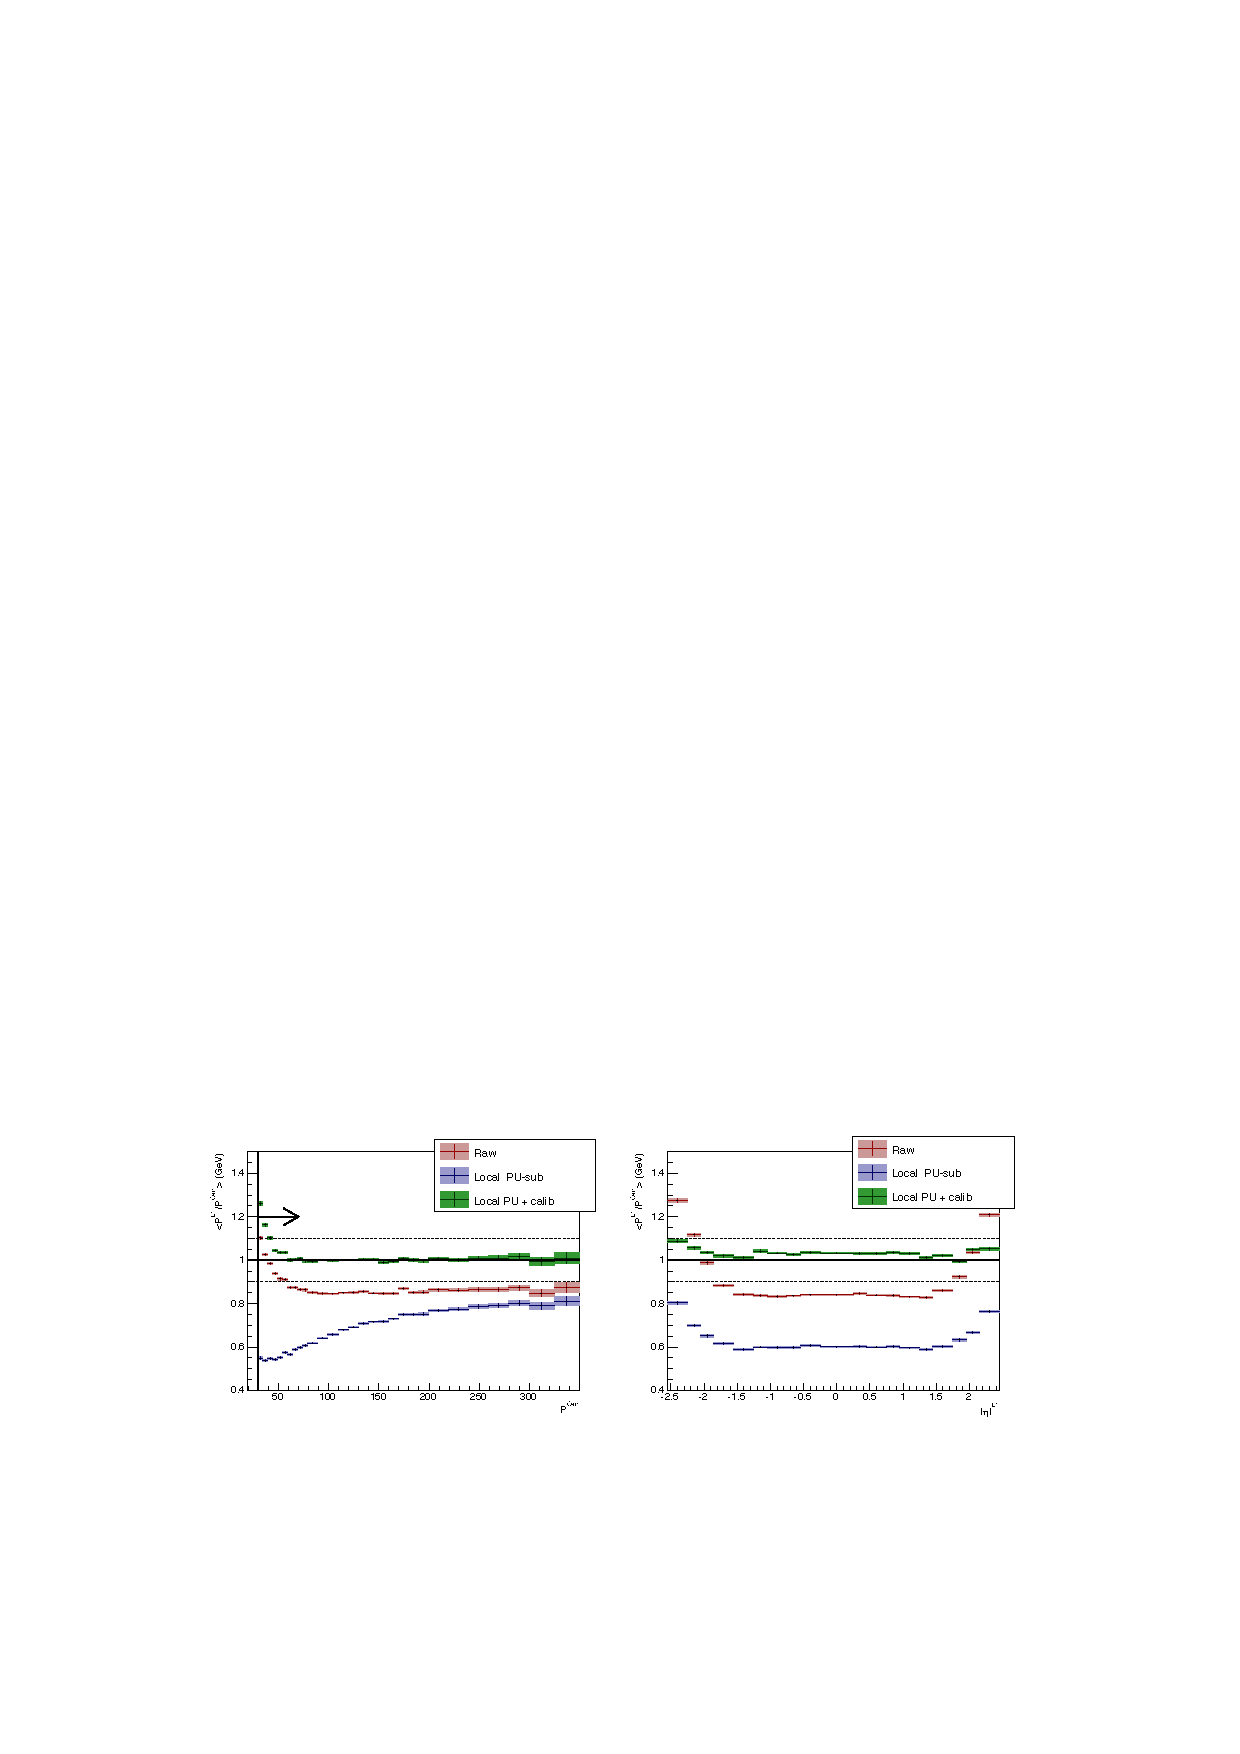
\includegraphics[width=1.0\linewidth]{figs/trigger/pu140_calib_closure}
  \caption{The ratio of L1 jets with Gen before and after they are calibrated,
demonstrating the effectiveness of the calibration}
  \label{fig:pu140calibclosure}
	\end{center}
\end{figure}

\section{Performance of the upgraded algorithm}

\label{sec:jet_algo_performance}

The performance of the jet algorithm with the various methods of \PUS 
described in Sec.~\ref{sec:pus} is tested on 13~TeV \MC simulation with an
average \PU of 40. A comparison is made to the jets produced by the
\GCT as it was in 2012. In some cases the performance of the interim
calorimeter trigger that was run in the early stage of 2015 during the
commissioning of the upgraded trigger is plotted with label
\emph{UCT}. To investigate rates a minimum bias sample was used, this
sample only consists of overlaid \PU events and has no generator jets.
To test physics performance a sample of simulated $t\bar{t}$
events was used, which contains generator jets that originate from
the hard interaction. The Level-1 jets jets are calibrated for each
type of \PUS with the method as outlined in Section~\ref{sec:l1jec}.

Fig.~\ref{fig:matchingeff} shows the efficiency of generator jets,
produced as described in Sec.~\ref{sec:l1jec}, being matched to a
Level-1 jet as a function of their $p_T$. If a generator jet has a
corresponding Level-1 jet within a radius $R=0.5$ it is counted as
matched.
This radius is chosen as the distance from the centre of a L1 jet to
the corner of its $9\times9$ square. A representative selection of the
different \PUS algorithms are shown. All of the upgrade Level-1 jet
algorithms have close to $100\%$ efficiency above $70$~GeV. The
application of a seed threshold significantly reduces the efficiency
for low $p_T$ jets, but the donut subtraction does not remove any
extra signal jets.
%Checked matching to gen, dr 32, inefficiencies caused by algorithm - gct bad
\begin{figure}
	\begin{center}
		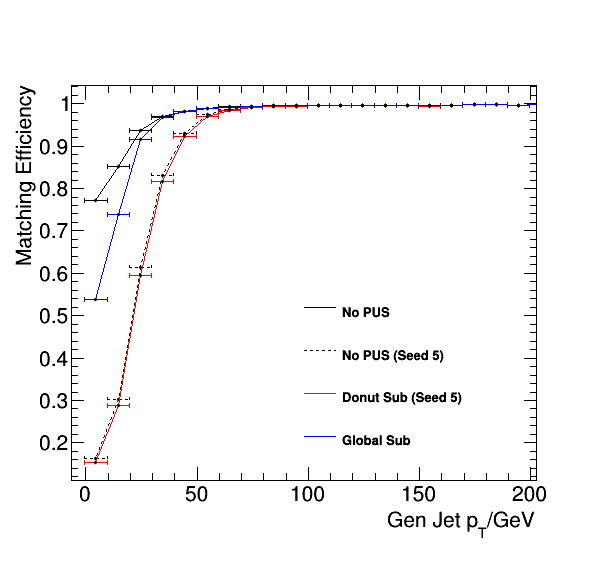
\includegraphics[width=0.6\linewidth]{figs/trigger/performance/matchingeff_alljet}
	\end{center}
	\caption{The efficiency with which a generator jet has a
  corresponding L1 jet within a radius, $R=0.5$. This is carried out
  for all Gen jets in 70~000 simulated $t\bar{t}$ production events.}
	\label{fig:matchingeff}
\end{figure}

A key goal of \PUS is to reduce the dependence of the Level-1 trigger
acceptance rate on the number of \PU interactions. To quantify this
for a representative selection of algorithms, the rate against the
number of reconstructed vertices is plotted for the minimum bias sample,
Fig.~\ref{fig:ratenvtx}. The rate is defined as the fraction of
minimum bias events that pass a Level-1 jet $p_T$ cut of $30$~\gev.
This cut is applied to a different jet rank depending on the type of
trigger to be tested. For \emph{single-jet} trigger the cut is applied to
the lead jet, for a \emph{quad-jet} trigger the cut is applied to the
fourth leading jet. The different forms of \PUS clearly reduce the
dependence of the rate on the number of interactions. The upgrade algorithm
performs significantly better than the \GCT, where the jet trigger
rates are incredibly sensitive to PU. Of the algorithms investigated,
the seed of 2.5~\gev, denoted \emph{Seed 5}, has the most dramatic
effect due to its ability to kill soft \PU jets. The \rho-area
subtraction, denoted \emph{Global Sub}, also performs well. Applying
donut subtraction without a seed threshold does not making much difference for this
particular \PUS benchmark. This is likely due to the fact that
donut subtraction works well in correcting the resolution of jets
contaminated with soft particles from \PU vertices, rather than
removing low \pT jets that originate from \PU.

\begin{figure}
  \centering
  \subfloat[Single-jet trigger $\pT>30~\gev$]{
    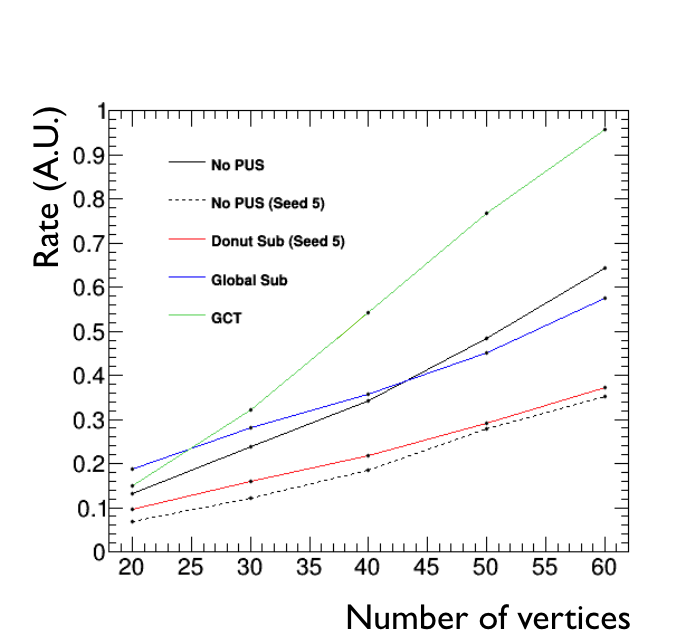
\includegraphics[width=0.5\textwidth]{figs/trigger/performance/rateNVertLeadJet}
  }~ 
  \subfloat[Quad-jet trigger $\pT>30~\gev$]{
    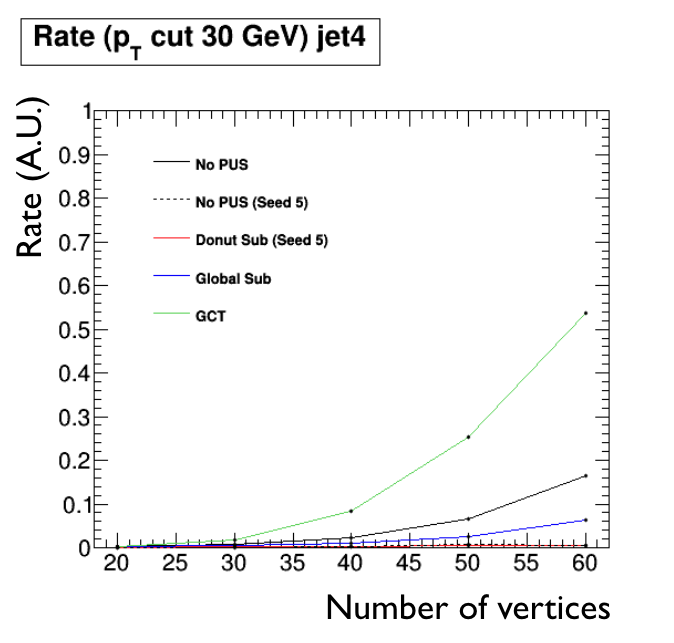
\includegraphics[width=0.5\textwidth]{figs/trigger/performance/rateNVertFourthJet}
  }
  \caption{The relative rate of events with $p_T>30$~GeV leading (a)
  and fourth leading (b) jets after different \PUS algorithms with and
  without seed thresholds for $70 000$ zero bias events as a function
  of the number of reconstructed vertices.}
  \label{fig:ratenvtx}
\end{figure}

To characterise the energy resolution of the Level-1 jets with
different \PUS algorithms, the efficiency turn-on curves are plotted
in Fig.~\ref{fig:turnons}. The lead jet efficiency turn-on,
Fig.~\ref{fig:leadJetTurnon}, is
made by matching the generator jets to Level-1 jets, requiring $\Delta
R<0.5$ and taking the ratio of the matched generator jet $p_T$
distribution without a cut on the Level-1 jet with the matched
generator jet distribution after a cut on the Level-1 jets. Most algorithms
show a similar performance for a single-jet trigger. The effects of
\PU are less relevant when just considering one high energy object.

More difference is observed when all jets with $\pT>20~\gev$ are
summed to find the Level-1 $\HT$ of the event. The plot in
Fig.~\ref{fig:htTurnon} is made by taking the ratio of generator $\HT$
(also made from 20~\gev jets), with and without a cut on the Level-1
\HT. When considering a scalar sum of jets the effects of pileup
add up and the different algorithms have a more significant
separation. It is clear that performing \PUS helps to significantly
improve the energy resolution of Level-1 $\HT$.
\begin{figure}
  \centering
  \subfloat[Lead jet $p_T^{L1}>150~\gev$ efficiency]{
    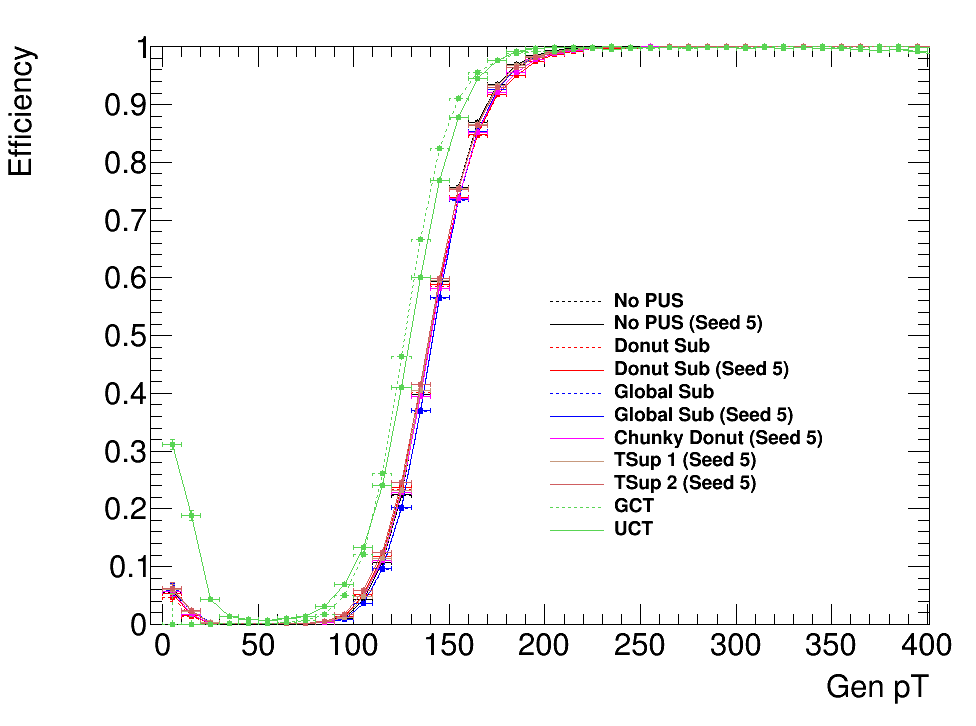
\includegraphics[width=0.515\textwidth]{figs/trigger/performance/leadJet_150_turnon}
    \label{fig:leadJetTurnon}
  }~
  \subfloat[$\HT^{L1}>200~\gev$ efficiency]{
    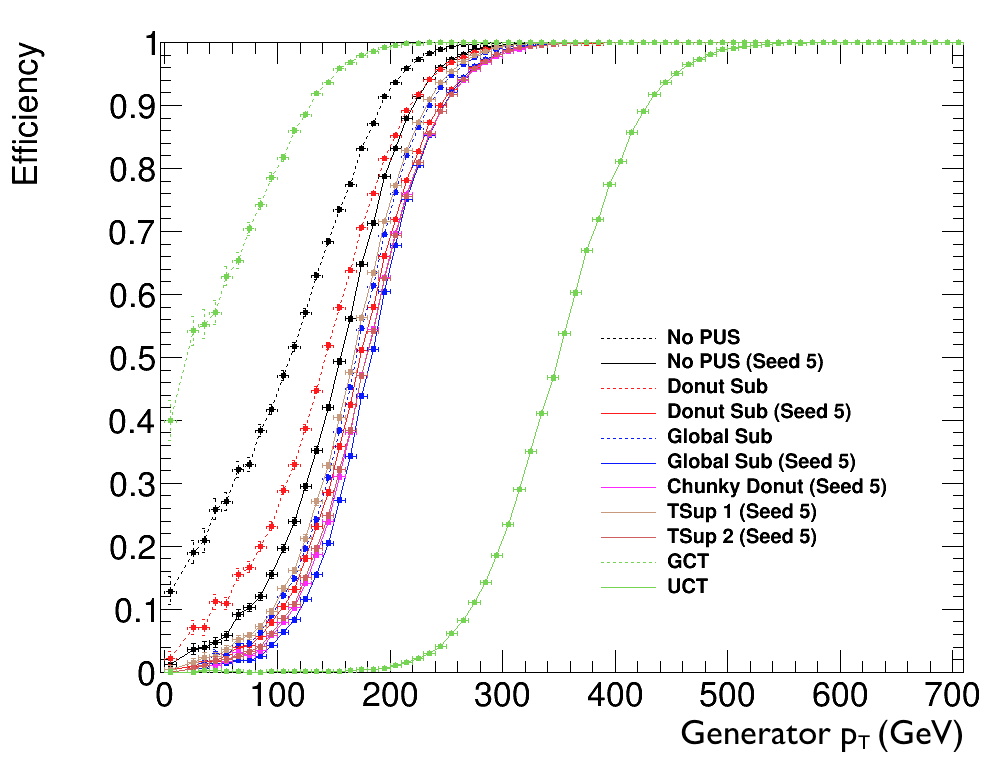
\includegraphics[width=0.485\textwidth]{figs/trigger/performance/ht_200_turnon}
    \label{fig:htTurnon}
  }
  \caption{ Efficiency after a specific cut for Level-1 leading jets (a) and Level-1 \HT
  (b) as a function of the corresponding generator quantity.
  } \label{fig:turnons}
\end{figure}

In the turn-on curves, a change in offset along the $x$-axis results
from a difference in jet energy scale with respect to the generator
quantity. As the \GCT jets do not have any calibration applied and the
UCT has a different type of calibration, this can differ
significantly. However, this does not give all the relevant
information when deciding on a final algorithm to increase the overall
performance of the trigger. The most important consideration is the
trade-off between the efficiency of the algorithm at picking out a
particular physics signature for a given rate. This does not depend on
the specific energy scale of the jets relative to the generator
quantities.

To better characterise the different Level-1 jet algorithms independently of energy
scale, the efficiency of selecting events with a particular generator
level jet quantity is plotted against the rate from a minimum bias
sample. In each case, a range of thresholds for the equivalent Level-1
quantity are scanned through and the rate and efficiency for that
threshold is plotted. The rate is calculated for an instantaneous luminosity
of $7\times10^{33}$~cm$^{-2}$s$^{-1}$ with a 50~ns \LHC bunch crossing
interval. Figure~\ref{fig:rateEffJet} shows the rate of the Level-1
trigger in Hz against the efficiency of selecting events for jet
triggers. In Fig.~\ref{fig:leadJetTurnon} the efficiency of
selecting $t\bar{t}$ events containing a generator jet with
$\pT>150~\gev$ is plotted against the minimum bias rate for an
equivalent Level-1 threshold. The rate and efficiency are plotted for
a range of cuts on the lead Level-1 jet for all the jet algorithms
discussed in this chapter. In Fig.~\ref{fig:fourthJetTurnon} the
efficiency of selecting events with a fourth leading generator jet
with $\pT>50~\gev$ are plotted for a range of cuts on the fourth Level-1
jet. As was observed in the turn-on curves, the efficiencies for the
lead jet triggers do not depend so much on the type of \PUS, although
there is a moderate improvement for all the upgrade algorithms over
that used in the \GCT. The difference becomes more evident when
considering the efficiency of selecting a fourth leading jet. The
lower \pT fourth leading jets show a more significant improvement with
the upgraded jet algorithm. The application of \PUS has some effect
but it is still not significant when just considering relatively high
$\pT$ and low multiplicity jets. The performance favours some form of
seed threshold, with the global \PUS performing slightly better than
the local variants.

Considering the jet triggers is important to understand the
behaviour of the upgraded algorithm for individual jets. However,
energy sum triggers are typically more widely used when searching for
signatures of \BSM physics with lots of hadronic activity and missing
energy. This is due to the fact that they give a total measure of the
hadronic energy scale of the event and a strong indication of the
presence of any weakly interacting particles. The performance of the
\HT and \MHT triggers is therefore of significant interest and shown
in Fig.~\ref{fig:rateEffJet}. In Fig.~\ref{fig:htTurnon} the
efficiency of selecting $t\bar{t}$ events with a scalar sum of $p_T>20~\gev$
generator jets that is greater than $200~\gev$ for a range of
thresholds on the Level-1 $\HT$ is plotted against the minimum bias
rate. When many jets are summed in this way the application of \PUS
makes a significant difference. Applying a seed threshold on the
selected jets performs well. Applying the chunky donut or
$\rho$-area \PUS methods on top of a seed threshold obtains the best result.

Figure~\ref{fig:mhtTurnon} shows a similar rate and efficiency curve
for the \MHT variable. For reference on this plot the \MET rate and
efficiency, labelled \emph{MET}, is also shown. As a
vector sum of jets is not made in the interim trigger, the curve with
the UCT label is a form of \MET constructed from \ac{RCT} regions. As \MET
uses the full granularity \TT information without any clustering it
has an improved resolution, but loses robustness as the inputs are not
calibrated and are more susceptible to influence from detector noise.
Of the rate and efficiency curves constructed from a vector sum of
jets, it is again observed that a seed threshold with chunky donut or
\rho-area \PUS give the best performance.

\begin{figure}
  \centering
  \subfloat[Lead jet $p_T>150~\gev$]{
    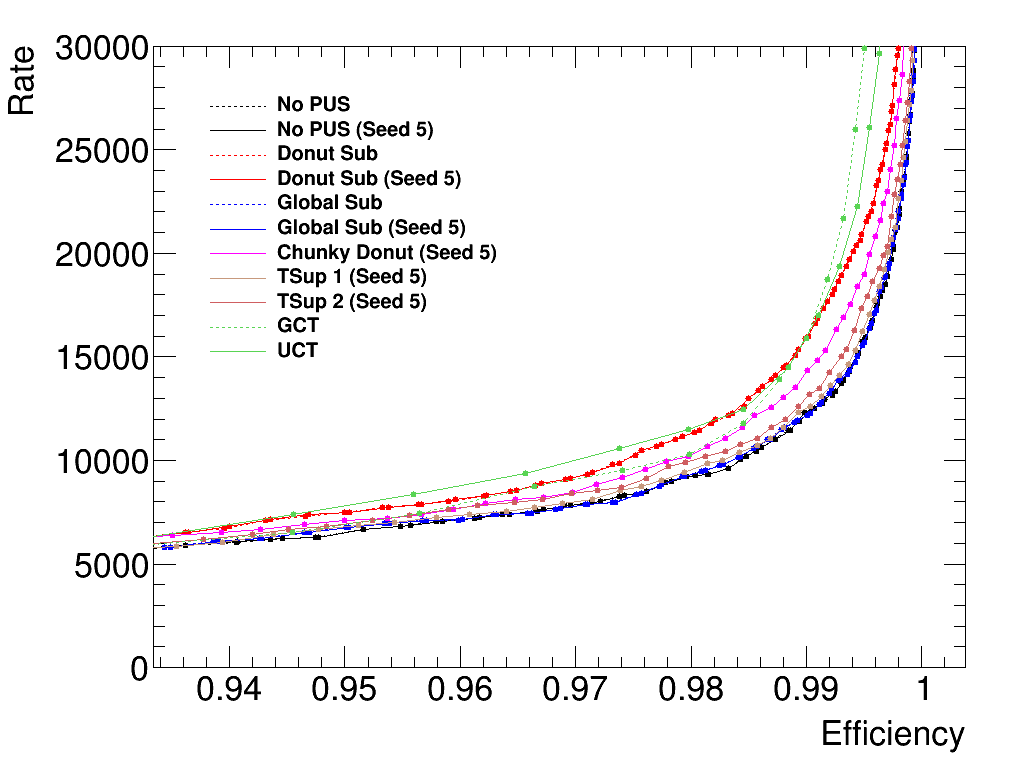
\includegraphics[width=0.48\textwidth]{figs/trigger/performance/singleJet_150}
    \label{fig:leadJetTurnon}
  }~ 
  \subfloat[Fourth leading jet $p_T>50~\gev$]{
    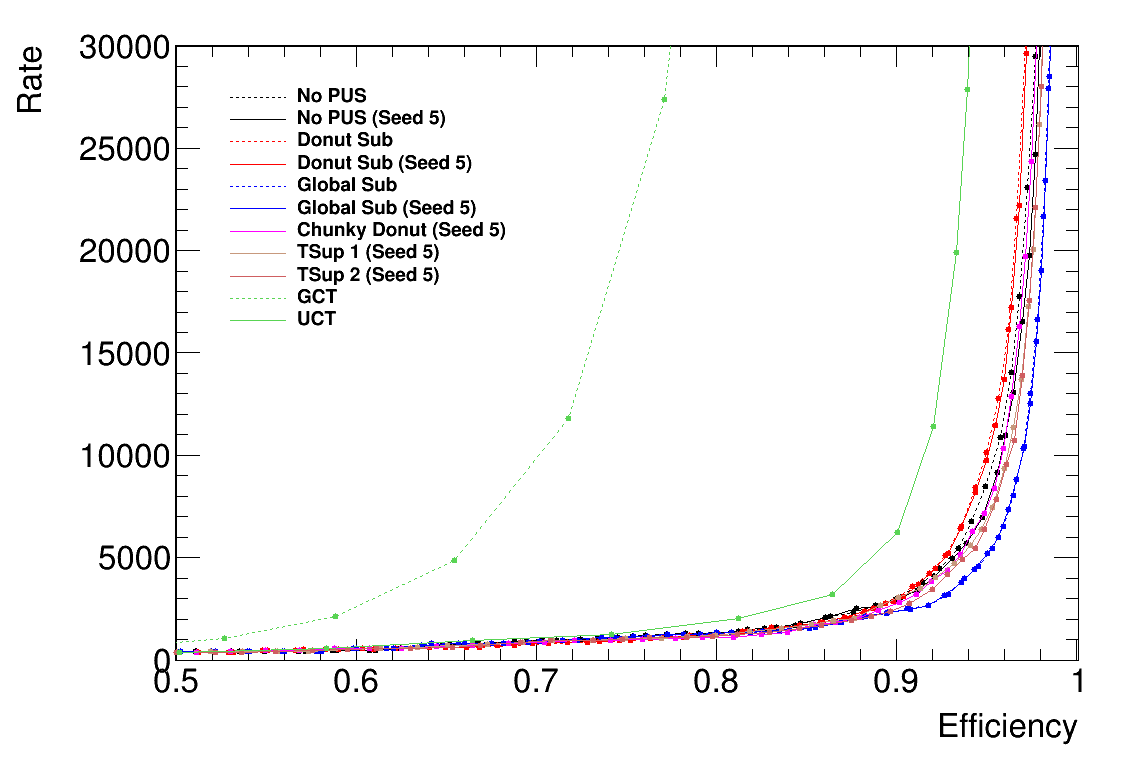
\includegraphics[width=0.52\textwidth]{figs/trigger/performance/quadJet_50}
    \label{fig:fourthJetTurnon}
  }
  \caption{ The normalised minimum bias rate (in Hz) against efficiency for a
  variety of thresholds of jet triggers
  made from jets with various \PUS schemes. Based on $t\bar{t}$ and
  minimum bias \MC simulation.}
  \label{fig:rateEffJet}
\end{figure}

\begin{figure}
  \centering
  \subfloat[$\HT>200~\gev$]{
    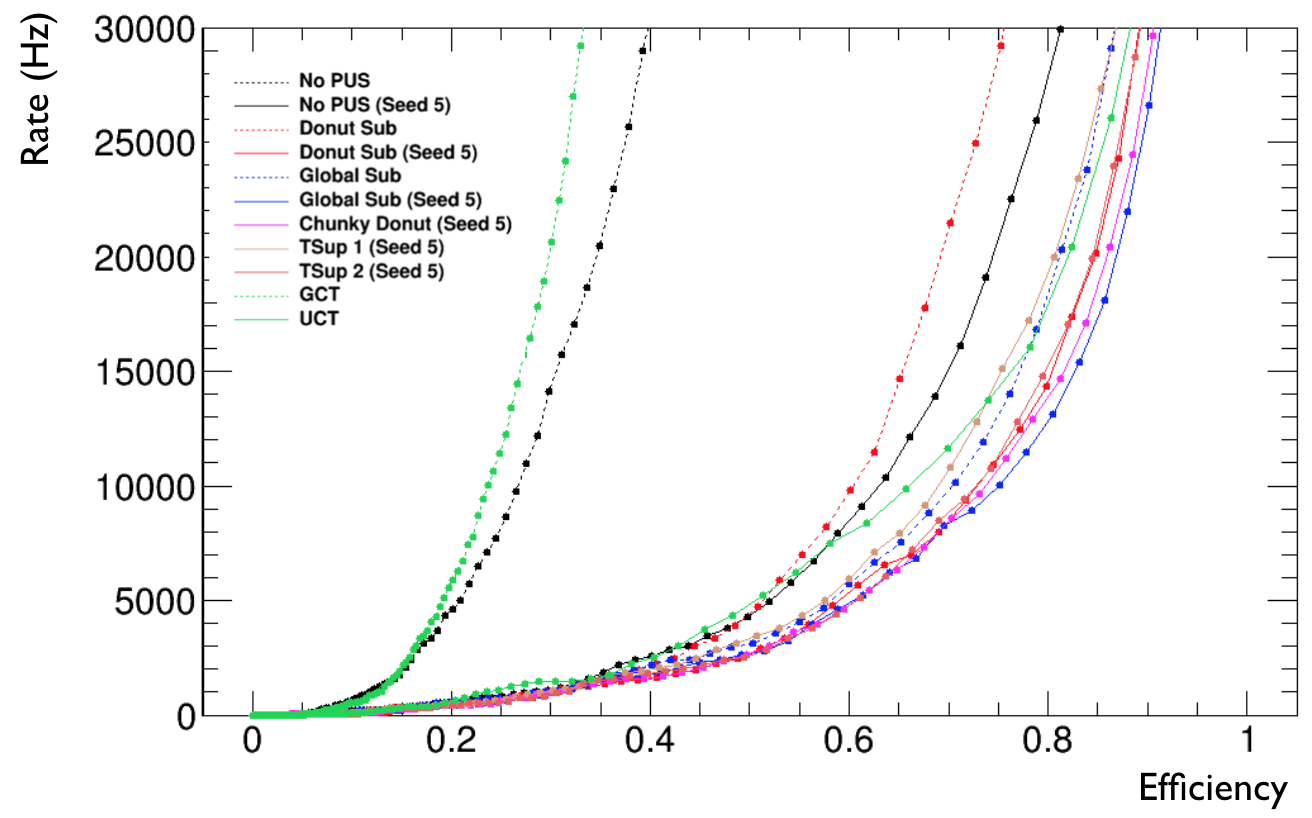
\includegraphics[width=0.5\textwidth]{figs/trigger/performance/ht_200}
    \label{fig:htTurnon}
  }~
  \subfloat[$\MHT>200~\gev$]{
    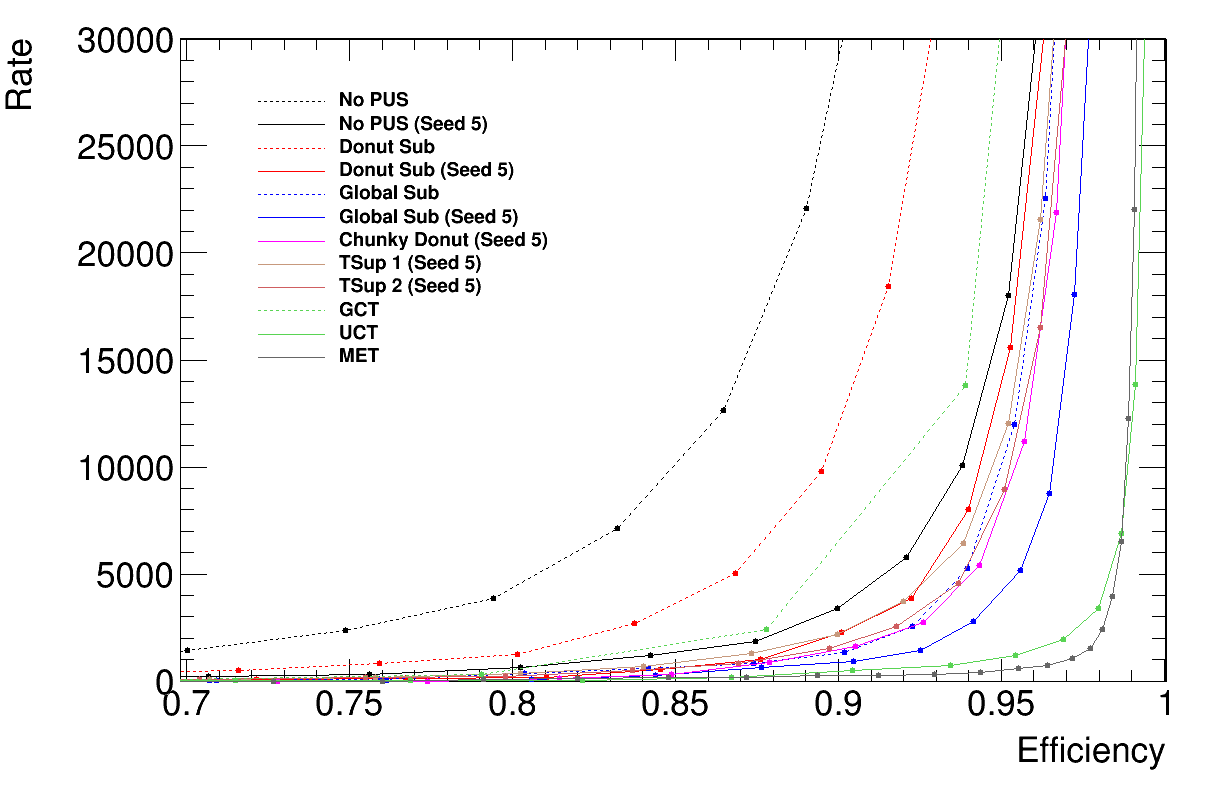
\includegraphics[width=0.5\textwidth]{figs/trigger/performance/mht_200}
    \label{fig:mhtTurnon}
  }
  \caption{ The normalised minimum bias rate (in Hz) against efficiency for a
  variety of thresholds of energy sum
  triggers made from jets with various \PUS schemes. Based on
  $t\bar{t}$ and minimum bias \MC simulation.}
  \label{fig:rateEffJet}
\end{figure}

\subsection{Conclusions}

After investigating the performance of the upgrade trigger algorithms
with simulation, it can be concluded that the upgrade algorithm
presents a significant improvement over the algorithm used in the \GCT
during Run~1 of the \LHC. The application of \PUS appears most useful
when summing jets to make trigger decisions. This is due to the fact
that \PU has the biggest effect on the energy of lower \pT jets from
the primary vertex and is most likely to produce low $\pT$ jets.
Overall, it can be inferred that the application of a seed threshold
effectively removes jets that originate from \PU. It is then possible
to successfully correct the energy of jets originating from the hard
scatter with both local and global \PUS methods. The chunky donut
algorithm performs most effectively for local \PUS. The $\rho$-area
form of \PUS seems to perform slightly better, but comes with
significant latency penalties when implemented in hardware. This is
particularly true when $\rho$-area \PUS is applied with a seed, as two
jet collections must be made, those with a seed and those without for
the $\rho$ calculation. Local forms of \PUS are also more robust
against localised detector faults, which can lead to issues with the
trigger inputs. With these considerations, it is concluded that the
$9\times9$ \TT jets with a 2.5~\gev seed threshold and chunky donut
\PUS is the most promising candidate for an upgrade algorithm. 

\section{Firmware emulation and testing}
\label{sec:emu}

After choosing a promising jet finder algorithm, it must be implemented
within the firmware of the \FPGA boards that will be used within the
Level-1 trigger. To provide a reference for validation of the
algorithm in firmware, a version is implemented in software, known as
the \emph{emulator}. The software is written to behave in a way that
is very close to the implementation in the \FPGA hardware. This
emulator is then included in the collaboration wide \emph{\CMS
software} and can be used to process data and simulation to produce an
emulated Level-1 trigger output. This is particularly useful when
testing the Level-1 trigger in simulation, for example when measuring
trigger efficiencies for a particular physics analysis. It is also
used to check that the Level-1 hardware is performing as expected
during the online data collection.

In the early stages of the firmware implementation, the jet finding
was validated against the algorithm in the emulator. A collection of
simulated events were processed by both the firmware within an \FPGA
and the emulator. After checking several of the jets were correctly
reconstructed by hand, the output of the firmware and emulator were
compared. As is shown in Fig.~\ref{fig:firmwareEmu}, the emulator and
firmware implementations both find jets in exactly the same positions
in the detector. These plots have a limited number of jets but demonstrate a first step towards a more
comprehensive validation of the emulator. This kind of testing was
extensively used to check the behaviour of the algorithm in the
firmware and to ensure the trigger decisions were properly emulated
in simulation.

\begin{figure}
  \centering
  \subfloat[]{
    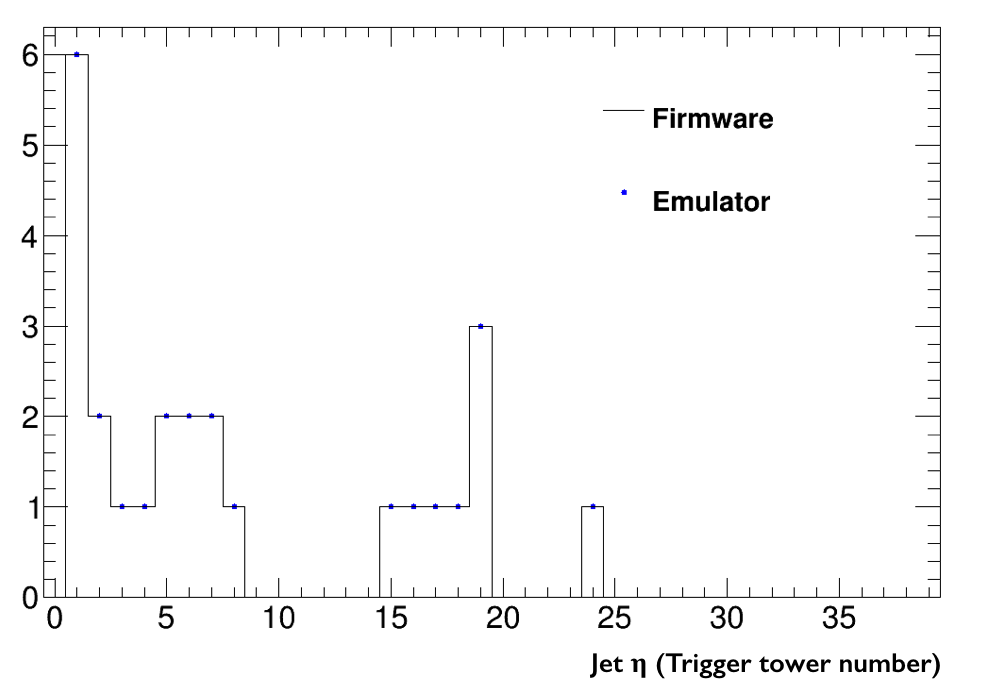
\includegraphics[width=0.48\textwidth]{figs/trigger/jetEtaEmulator}
    \label{fig:leadJetTurnon}
  }~ 
  \subfloat[]{
    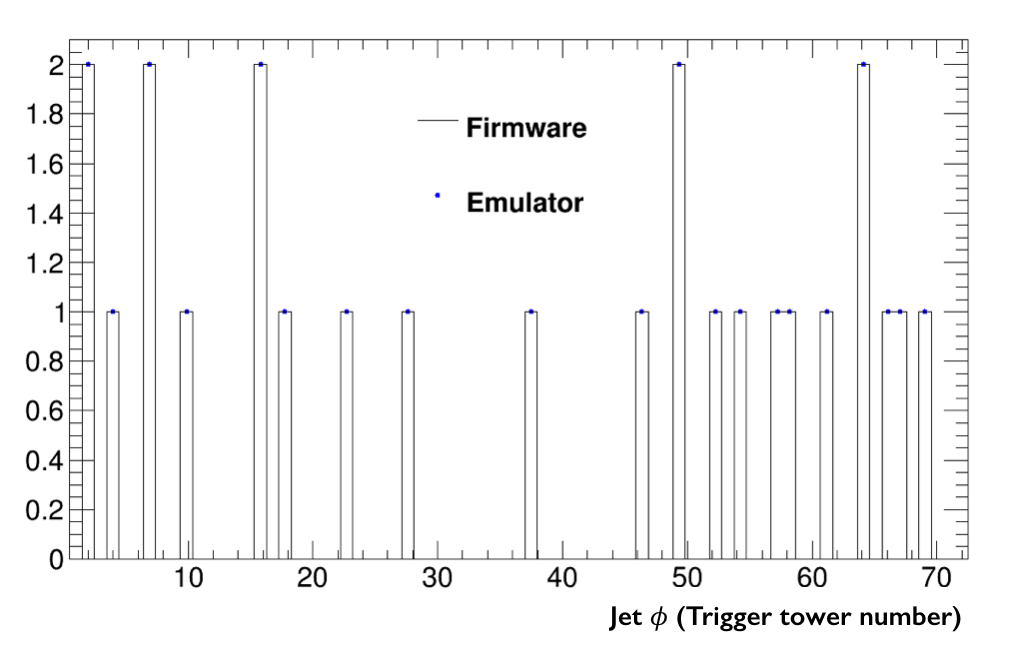
\includegraphics[width=0.52\textwidth]{figs/trigger/jetPhiEmulator}
    \label{fig:fourthJetTurnon}
  }
  \caption{Demonstration of agreement between the trigger algorithm
  implemented in firmware and emulated in software for simulation
  studies}
  \label{fig:firmwareEmu}
\end{figure}

The chunky donut $9\times9$ \TT jet finder algorithm has been fully
implemented into the upgrade hardware and successfully tested. It was
commissioned throughout the data collection during 2015 and has been
used to make the Level-1 trigger decisions when collecting data during
Run~2 from 2016 onwards.

%%% EXTRA PERFORMANCE STUFF FROM 9 MNTH THAT ISNT RELEVANT:

% The other purpose of PUS is to correct the energy of L1 jets
% contaminated with PU. The resolution of the jets as compared to Gen is
% defined as $\frac{p_T^{L1}-p_T^{Gen}}{p_T^{Gen}}$, being zero for
% perfect agreement. The PUS should act to remove the dependence of the
% resolution on the number of interactions in an event. In
% Figure~\ref{fig:resolution} it can be seen that the donut and global
% $\rho$ subtraction do flatten out the resolution for a representative
% bin of $p_T$ and $\eta$, whereas the seed on its own does not. 
% \begin{figure}
% 	\begin{center}
% 		\includegraphics[width=0.6\linewidth]{performance/pt_20to40_eta_-28to-14}
% 	\end{center}
% 	\caption{The resolution of L1 jets with $20<p_T<40$~GeV and with $-3<\eta<-1.2$ as a function of the number of interactions (NVTX)}
% 	\label{fig:resolution}
% \end{figure}
%correcting hard jets- response

% As a final performance test, the $H_T$ and $\cancel{H}_T$ as defined
% in Section~\ref{sec:alphaT} are plotted. If the PUS is too aggressive
% the $H_T$ will be too low when compared to Gen, or too high if it
% under subtracts. Figure~\ref{fig:htmht} shows that jets with a seed
% threshold most closely reproduce the $H_T$. Overall the PUS methods
% are under subtracting, however. The PUS does not improve the
% $\cancel{H}_T$ distribution, this is expected in the case that PU is
% distributed evenly.
% % \begin{figure}
% % 	\begin{center}
% % 		\includegraphics[width=0.5\linewidth]{performance/ht_ttbar}\put(-42,203){(a)}
% % 		\includegraphics[width=0.5\linewidth]{performance/mht_ttbar}\put(-42,203){(b)}
% % 	\end{center}
% % 	\caption{(a) The distribution of the total energy of jets in each event ($H_T$). (b) The distribution of the missing momentum of jets in an event ($\cancel{H}_T$).}
% % 	\label{fig:htmht}
% % \end{figure}
% %not killing important jets- ht mht
